%\documentclass[final,authoryear,1p]{elsarticle}
%\documentclass[final,authoryear,5p,times,twocolumn]{elsarticle}
\documentclass[authoryear,preprint,review,9pt]{elsarticle}
\usepackage{amssymb}
\usepackage{amsmath}
\usepackage{bbm}
\usepackage{graphicx}
\usepackage{subfig}
\usepackage{algorithmic}
\usepackage{algorithm}
\usepackage{relsize}
\usepackage{booktabs}
\usepackage{color}
\usepackage[labelfont={small,bf}]{caption}
\usepackage[font={small,bf}]{caption}
\usepackage[margin=1.0in]{geometry}
\newcommand{\closer}{\vspace{-0.2cm}}

\journal{Medical Image Analysis}

\begin{document}


\begin{frontmatter}

\title{\textbf{Symmetric Diffeomorphic Registration with Expected Cross-Correlation for Multi-Modal MRI}}
\author[cimat]{Omar Ocegueda\corref{cor1}}
\ead{jomaroceguedag@gmail.com}
\cortext[cor1]{Corresponding author}

\author[scil]{Eleftherios Garyfallidis}

\author[scil]{Maxime Descoteaux}

\author[cimat]{Mariano Rivera}

\address[cimat]{Centro de Investigaci\'{o}n en Matem\'{a}ticas, Guanajuato, Gto, M\'{e}xico}
\address[scil]{Computer Science Department, Universit\'{e} de Sherbrooke, Sherbrooke, Qu\'{e}bec, Canada}

\begin{abstract}
    We present a new algorithm for multi-modal symmetric diffeomorphic image registration. The transfer functions between the two modalities are modeled as a set of hidden variables, which results in a metric that may be regarded as a generalization of the correlation ratio. We apply the greedy symmetric image normalization method (SyN) to efficiently maximize the image similarity metric in the space of diffeomorphic transformations. We validate our algorithm using the publicly available IBSR database and the Brainweb synthetic template, obtaining very competitive results in both mono- and multi-modal image registration. As a natural extension, we generalize the widely used
    normalized cross correlation metric, for multi-modality images, and show that the resulting metric, which we call expected cross correlation, performs better than the original cross correlation in the multi-modal case, without reducing performance in the mono-modal case.
\end{abstract}


\begin{keyword}
Multi-modal registration \sep Deformable registration \sep Diffeomorphic \sep Expectation maximization \sep Cross-correlation
\end{keyword}

\end{frontmatter}


\section{Introduction}
The human brain has been a subject of extensive research by the medical image community with a wide range of objectives, from practical clinical applications like disease diagnosis and surgical planning, to addressing scientific questions related to its structure and functionality. The goal of brain image registration is to compute a transformation that brings images of the brain into anatomical correspondence so that they can be jointly analyzed. A rough classification of volumetric image registration methods may be based on two main criteria: a) the deformation model (linear/non-linear), and b) the similarity measure (mono-modal/multi-modal). Registration of images from different modalities (\emph{multi-modal} image registration) is a specially challenging task, since an appropriate similarity metric is harder to define in the multi-modal case than in the \emph{mono-modal} case. Multi-modal image registration has traditionally been constrained to linear methods: since registration of medical images of different modalities is almost exclusively applied to intra-subject image registration, it is often believed that there must exist a linear transformation that correctly brings them into correspondence. However, certain imaging modalities present severe distortions that cannot be accommodated by a linear model. Diffusion MR images, for instance, suffer from distortions caused by $B_{0}$ susceptibility and eddy-currents \citep{Tournier2011, Andersson2003}, which makes their registration to other modality images, even from the same subject, a non-linear problem if these artifacts are not corrected beforehand. Despite the complexity of the task, multi-modal image registration has a wide range of potential applications. Combining diffusion data with T1 MRI, for instance, has the potential of significantly improving tractography \citep{Smith2012, Girard2014}.

\subsection{Multi-modal registration using information theoretic measures}
Existing multi-modal registration methods may be classified into two main approaches: 1) those that optimize information theoretic measures from the estimated joint probability distribution, 2) those that reduce the multi-modal problem to the mono-modal case. The most prominent example of metrics based in information theory is mutual information (MI) \citep{Maes1997, Mattes2003}. The success of MI is explained by its generality, since it does not assume the existence of a functional relationship between the intensities in the two modalities. This generality comes at the expense of disregarding any notion of proximity of intensity values: two intensities will be considered similar only if their estimated joint probability is high, no matter how close they are numerically, which may cause a large number of local maxima \citep[see][Fig. 2]{Roche1998}. In the standard formulation of MI, the joint probability distribution is estimated from the whole image ({\it i.e.}, it is a {\it global} metric), which makes the metric more robust to the effects of noise \citep{Mattes2003}. An important limitation of this kind of global metrics is precisely that the metric depends solely on the (globally) estimated probability distribution, which cannot capture non-stationary relationships between the image intensities \citep{Hermosillo2004}. Since the probability distributions relate point-wise intensity values (intensities of individual voxels), the metric is also insensitive to local image features that are important in non-linear registration like edges and texture \citep{Heinrich2012}. As pointed out by \cite{Sotiras2013}, any random spatial permutation of corresponding pixels would result in exactly the same distribution. A direct approach to tackle the problem of non-stationary intensity dependencies is to use locally estimated probability functions. \cite{Hermosillo2004}, for instance, uses Gaussian kernels centered at each voxel as weighting functions to reduce the contribution of far voxels to the local distribution. A limitation of using Gaussian kernels is the computational cost, as pointed out by \cite{Hermosillo2004}, which makes it necessary to perform some simplifications and use parallel computing. Besides, as we reduce the number of local samples, the estimation becomes more sensitive to noise~\citep{Mattes2003}.

\subsection{Multi-modal registration by reduction to the mono-modal case}
Reducing the multi-modal problem to the mono-modal case may be accomplished by assuming the existence of a {\it transfer function} between the two modalities (a function that maps intensity values of one modality to corresponding intensities in the other). \cite{Roche2000} showed that, assuming the existence of a transfer function, a maximum-likelihood formulation of the registration problem is equivalent to maximization of the correlation ratio (CR). The main drawback of CR is precisely that it relies on the strong assumption of a functional dependency between the two modalities, which in general is not satisfied. However, experimental results have shown that this assumption is not critical for typical brain image registration tasks~\citep{Roche1998}. Being a global metric, CR shares the robustness to noise of MI but also the inability to capture non-stationary relationships between image intensities. However, one of the advantages of CR over MI is that it is sensitive to proximity of intensity values, which may help to reduce the number of local maxima \citep{Roche1998}. An additional advantage is that the CR metric can be computed efficiently from statistics from the images' iso-sets instead of explicitly estimating the joint distribution. Recently, \cite{Arce-santana2014} proposed a similar formulation of the registration problem which also uses the functional dependency assumption. In their work, the transfer function is modeled as a set of hidden random variables whose values can be estimated using the Expectation Maximization (EM) algorithm. Since the assumptions are similar to those made by \cite{Roche1998, Roche2000}, the resulting optimal transfer functions are the same. However, the resulting metric (which is also obtained by maximum-likelihood estimation) differs in that it introduces a measure of uncertainty in the estimated transfer function for each intensity value. This uncertainty appears in the metric as a weighting function that controls the contribution of each voxel intensity, and it helps to alleviate the effect of non-functional and non-stationary dependencies between the two modalities. One of the limitations of the original formulation proposed by \cite{Arce-santana2014} is that it is asymmetric (a limitation shared with the CR metric) in the sense that the transfer function to be estimated must be chosen beforehand (notice that there are in fact two transfer functions mapping intensities from one modality to the other), which may result in very different solutions. Another limitation is that \cite{Arce-santana2014} use an elastic deformation model \citep{Bajcsy1982, Gee1999}, and their optimization strategy consists in a Gauss-Newton iterative algorithm \citep{GVK502988711} that requires to solve a series of large systems of linear equations.

\subsection{Quantitative evaluation}
Besides developing deformation models and metrics, validation is one of the most challenging aspects in image registration. The most accepted validation methodologies, in the mono-modal case, consist in measuring the overlap of manually annotated anatomical regions \citep{Klein2009, Klein2010, Rohlfing2012}. These methodologies have made possible to quantitatively evaluate non-linear registration algorithms and compare their performance in a meaningful way. The Symmetric Normalization (SyN) algorithm developed by Avants {\it et al.}, and made available as part of the Advanced Normalization Tools (ANTS), has been extensively tested in large comparative studies using the aforementioned methodologies and has consistently been reported as one of the most accurate. For multi-modal images, the MI metric is implemented in ANTS, and can be used with SyN for diffeomorphic registration. However, to the best of our knowledge, there are no equivalent studies that quantitatively evaluate the accuracy of non-linear registration algorithms in the multi-modal case, and performance is assessed, in practice, only visually. The reason why validation becomes more challenging in the multi-modal case is that, as far as we know, there are no manually annotated multi-modal image sets publicly available.

\subsection{Summary of contributions}
In this work, we propose an extension to the EM framework proposed by \cite{Arce-santana2014} in a symmetric fashion to simultaneously consider both transfer functions between image modalities. In addition, we minimize the resulting metric in the space of diffeomorphic transformations by using the symmetric diffeomorphic registration framework developed by \cite{Avants2008, Avants2011}. Our optimization strategy is based on Vercauteren's analysis of the \textit{diffeomorphic demons} algorithm \citep{Vercauteren2009} that may be regarded as a Generalized EM algorithm (GEM) \citep{Neal1998}, in which the energy is not fully optimized at each step with respect to the transformations but only reduced at each iteration. As a natural extension, we propose a new metric, called expected cross-correlation, which extends the cross-correlation metric for multi-modal images by taking advantage of the (globally) estimated transfer functions, which makes the estimation robust to noise, while at the same time achieving sensitivity to local features, captured by the cross-correlation computed over local windows. For quantitative evaluation, we propose a validation methodology for multi-modal brain MRI registration methods based on generating semi-synthetic images using real, manually annotated, mono-modal brain images and a synthetic multi-modal template.\\

In summary, our contributions are three-fold: 1) we extended the expectation maximization (EM) framework proposed by \cite{Arce-santana2014} in a symmetric fashion and minimize the resulting metric in the space of diffeomorphic transformations 2) we propose a new metric, called expected cross-correlation, which extends the cross-correlation metric for multi-modal images, and 3) we propose a quantitative validation methodology for multi-modal brain MRI registration methods.

\section{Background}

We regard an image $I$ as a function that maps voxels of a rectangular grid \hbox{$\mathcal{L}$}, of dimensions $n_{x} \times n_{y} \times n_{z}$ cells, to a set $G$ of
possible values called the ``dynamic range'' of $I$. The images we are interested in represent objects in physical space. This means that each point $(i,j,k)$ in the
3-dimensional grid $\mathcal{L}$ is associated to a point $(x,y,z) \in \Omega \subset \mathbf{R}^{3}$. When the coordinates of a point
\hbox{$(i,j,k)$} are not integers, the image can still be evaluated at $(i, j, k)$ by interpolation provided
\hbox{$(i,j,k) \in \left[0, n_{x}-1\right] \times \left[0, n_{y}-1\right] \times \left[0, n_{z}-1\right]$}, we denote this ``extended'' dense domain by using the bar decorator:
$\bar{\mathcal{L}}$.\\

The function that maps voxel coordinates of a grid $\mathcal{L}$ to their corresponding coordinates in physical space is an invertible affine transformation. Whenever we talk about
a grid $\mathcal{L}$ we implicitly assume that this $\mathcal{L}$ is associated to a specific grid-to-space affine transformation.
Since our images represent objects in physical space, and these objects are not tied to any specific grid, the same object may be sampled over any grid $\mathcal{L}$. Since
the grid-to-space transformation is invertible, we can, and will, unambiguously talk about images defined in physical space $\Omega \subset \mathbf{R}^{3}$.\\

\subsection{Symmetric diffeomorphic registration}

The goal of image registration is to compute a transformation $\phi: \Omega \rightarrow \Omega$ that brings a moving image $J:\Omega \rightarrow G$ into correspondence
with a fixed image $I:\Omega \rightarrow G$. The transformation $\phi$ is chosen from a set $\Phi$ of feasible solutions having properties that are desirable depending on the
application, such as smoothness and invertibility. Correspondence between $I$ and $J$ is defined to be reached when a dissimilarity metric between them is minimized.\\

In non-linear image registration, the transformation $\phi$ is usually represented by a deformation field $\mathbf{u(\cdot)}$ that assigns a displacement vector
to each point $x$ such that $\phi(x) = x + \mathbf{u}(x)$. The classical elastic model is one of the earliest formulation for non-linear image registration \citep{Bajcsy1982, Gee1999},
and may be written as

\begin{equation}\label{eq:elastic}
    \mathbf{u}^{*} = \arg \min_{\mathbf{u}} \int_{\Omega} ||L \mathbf{u}(x)||^{2}dV + \Pi(I, J \circ \phi),
\end{equation}
where $L$ is a differential operator used to promote smoothness on $\mathbf{u}$ and $\Pi$ is the dissimilarity metric driving the registration. A limitation of this model, especially important for medical image registration is that the solution, although being smooth, is not guaranteed to be invertible, and the topology of the moving image is not guaranteed to be preserved after transforming it under $\phi$.\\

To overcome the limitations of the elastic model, the large deformation proposed by \cite{Christensen2001} and further developed by \cite{Science2005} formulates the problem in terms of a trajectory of transformations \hbox{$\phi:\Omega_{I} \times [0, 1] \rightarrow \Omega_{J}$} that satisfies $\frac{d \phi(x, t)}{dt} = v(\phi(x, t), t)$ and $\phi(x, 0) = x$, where $v(\cdot, \cdot)$ is
the velocity field associated to the curve $\phi$. Beg's Large Deformation Diffeomorphic Metric Mapping (LDDMM) \citep{Science2005} formulation of the registration problem is given by:
\begin{equation}\label{eq:LDDMM}
    v^{*} = \arg \min_{v:\dot{\phi} = v_{t}(\phi)} \int_{0}^{1} ||L v_{t}||^{2} dt + \Pi(I, J \circ \phi(\cdot, 1)),
\end{equation}
where $\dot{\phi} = \frac{d\phi}{dt}$, $v_{t} = v(\cdot, t), t\in [0, 1]$. The final diffeomorphisms can be obtained by integrating over time
\begin{equation}\label{eq:velocity_integral}
    \phi(x, 1) = \phi(x, 0) + \int_{0}^{1}v(\phi(x, t), t) dt.
\end{equation}

\cite{Dupuis1998} showed that by enforcing sufficient smoothness in $v$, through the differential operator $L$, it can be guaranteed that $\phi(\cdot, t), t \in [0, 1]$ are diffeomorphisms. This and other formulations also based on diffeomorphic flows ensure that images are smoothly transformed and their topology preserved: an important property for many medical applications. \cite{Avants2008, Avants2011} modified the standard LDDMM formulation to enforce symmetry in the sense that the registration result is the same regardless of which image we designate as $I$ and $J$. This property, although natural and desirable, is not ensured in standard computational methods solving the LDDMM problem. By splitting the trajectory $\phi$ into two trajectories with opposite direction $\phi_{1}(x, t) = \phi_{2}(y, 1-t)$, where $y = \phi(x, 1)$, with corresponding velocity fields $v_{1}, v_{2}$, the Symmetric formulation for Diffemorphic Image Registration \citep{Avants2008, Avants2011} can be written as:

\begin{equation}\label{eq:syn_energy}
    \begin{array}{lll}
        v_{1}^{*}, v_{2}^{*} &=& \mathlarger{\arg \min \int_{t=0}^{0.5} ||L v_{1}(x, t)||^{2} + ||L v_{2}(x, t)||^{2} dt}\\
        &+& \mathlarger{ \Pi(I \circ \phi_{1}(\cdot, 0.5), J(\phi_{2}(\cdot, 0.5)))}
    \end{array}
\end{equation}
subject to
\begin{equation}\label{eq:syn_energy_constraints}
    \begin{array}{l}
        \frac{d\phi_{i}(x, t)}{dt} = v_{i}(\phi(x,t),t)\\
        \phi_{i}(\cdot, 0) = \mathbf{I},\, \phi_{i}^{-1}(\phi_{i}) = \mathbf{I},\, \phi_{i}(\phi_{i}^{-1}) = \mathbf{I},\, i=1,2,
    \end{array}
\end{equation}
where $\mathbf{I}$ denotes the identity transformation. \cite{Avants2006} proposed a numerical algorithm, called \textit{Geodesic SyN} for solving \eqref{eq:syn_energy}, which deforms both images towards the midpoint of the trajectory. The main drawback of directly solving eq. \eqref{eq:syn_energy} is its computational cost, since it requires space and time discretization and it is necessary to integrate the velocity fields in eq. \eqref{eq:velocity_integral} to obtain the trajectories at each iteration. A more efficient optimization algorithm to approximately solve eq. \eqref{eq:syn_energy}, also proposed by \cite{Avants2008, Avants2011}, consists in computing the gradient of the metric only at the midpoint of the trajectory (as opposed to evaluating it for all time):
\begin{equation}\label{eq:grad_metric}
    \nabla_{\phi_{i}} \Pi(\tilde{I}, \tilde{J}) = \frac{\partial}{\partial \phi_{i}} \Pi \left( \tilde{I}, \tilde{J}\right),
\end{equation}
where $\tilde{I} = I \circ \phi_{1}^{-1}(\cdot, 0.5)$, $\tilde{J} = J \circ \phi_{2}^{-1}(\cdot, 0.5)$. The midpoint diffeomorphisms are then updated by composition with the gradient after smoothing with a Gaussian kernel $K_{\sigma}$ (as opposed to integrating along the full geodesic)

\begin{equation}\label{eq:gsyn_update}
    \phi_{i}(\cdot, 0.5) = \phi_{i}(\cdot, 0.5) - \left( \epsilon K_{\sigma} \ast \nabla_{\phi_{i}} \Pi(\tilde{I}, \tilde{J}) \right) \circ \phi_{i}(\cdot, 0.5),
\end{equation}
where $\ast$ denotes the convolution operator and $\epsilon$ is a small factor controlling the step size in the optimization process. Finally, the updated midpoint transformations (which, after composition with the gradient, are not ensured to be diffeomorphisms) are forced to be invertible by using an explicit vector field inversion algorithm \citep{Chen2008}. This algorithm, called \textit{Greedy SyN} (see \ref{ap:Algorithms}, alg. \ref{alg:Greedy_SyN}) has been adopted by the neuroimaging community as the \textit{de facto} state-of-the-art brain MRI registration algorithm due to its reliability and efficiency. It was the method used for evaluating ANTS \citep{Avants2011} in the large comparative studies developed by \cite{Klein2009, Klein2010} in which \textit{Greedy SyN} consistently ranked first.

\subsection{Multi-modal image registration}

Defining an adequate similarity metric is arguably the most important aspect of image registration, and has been the subject of significant amount of research \citep{Sotiras2013}, if the minimum of the metric does not coincide with what we understand by optimal image correspondence, then no matter what transformation or optimization algorithm we choose, we are unlikely to correctly align the images. For mono-modal image registration, the Sum of Squared Distances (SSD) is used as a starting point for studying new transformation methods due to its simplicity, while Normalized Cross-Correlation (CC) is known to perform well in a larger number of applications since it compares local neighborhoods (as opposed to single voxel values used by SSD), which allows us to implicitly compare beyond voxel-level features.\\

Recently, \cite{Arce-santana2014} modeled the transfer function between the image modalities as
\begin{equation}\label{eq:arce_model}
    F[I(x)] = J(\phi(x)) + \eta(x), x\in \mathcal{L}
\end{equation}
where $F$ is the (unknown) transfer function between image modalities and $\eta(x), x\in \mathcal{L}$ are independent random variables with Gaussian distribution. To simplify
the problem, the dynamic range $G$ of image $I$ is assumed to be discrete and relatively small (\cite{Arce-santana2014} chose $G = \mathrm{Z}_{256}$). By having a discrete
dynamic range, the function $F: G \rightarrow G$ may be modeled as a discrete set of hidden random variables $Y_g = F(g), g\in G$ whose distribution parameters
can be estimated using the Expectation Maximization (EM) algorithm \citep{Dempster1977}. In their work, \cite{Arce-santana2014} used a discretized elastic
deformation model to test the behavior of their metric, which leads to the following energy minimization problem

\begin{equation}\label{eq:arce_elastic}
    \mathbf{u}^{*} = \arg \min_{\mathbf{u}} \sum_{x \in \mathcal{L}} \frac{1}{2 \sigma(x)^{2}} ( \bar{I}(x) - J(x + \mathbf{u}(x)))^{2} + \lambda \sum_{<x, y>} ||\mathbf{u}(x) - \mathbf{u}(y)||^{2},
\end{equation}
where $\bar{I}(x), \sigma(x), x\in \mathcal{L}$ are the estimated parameters (mean and standard deviation) of the hidden variable $F[I(x)]$ given the
observed intensity $I(x)$ and $<x, y>$ denote neighboring pixels in $\mathcal{L}$. Even though the authors only evaluated their metric for 2D image registration and used
the elastic model, this formulation can be extended, as we will show in the next section, to develop an efficient and accurate symmetric diffeomorphic non-linear image registration algorithm for 3D multi-modality data by taking advantage of the ideas of Avants' \textit{Greedy SyN} \citep{Avants2008}, Vercauteren's \textit{Diffeomorphic Demons} \citep{Vercauteren2009}and Arce's \textit{EM transfer function} model \citep{Arce-santana2014}.\\

\section{Methods}
\subsection{Bidirectional transfer functions model for multi-modal registration}\label{sec:syn_em}

Let $I$, $J$ be two images defined over $\Omega_{I}$, $\Omega_{J}$, respectively. We consider $\Omega_{I}, \Omega_{J}$ as the transformed grids $\mathcal{L}_{I}$, $\mathcal{L}_{J}$ associated to $I, J$, under their corresponding grid-to-space transforms $\mathcal{A}_{I}$, $\mathcal{A}_{J}$ (Fig. \ref{fig:syn_overview}). Let $G$ be the set of possible intensity values these images may take (e.g. $G=\left\lbrace 0,1,...,255\right\rbrace$). We aim to find two diffeomorphisms $\phi_{I}:\Omega_{I}\rightarrow \Omega_{R}$ and $\phi_{J}:\Omega_{J}\rightarrow \Omega_{R}$ such that the images get aligned in the reference space $\Omega_{R}$ after warping them under $\phi_{I}^{-1}$ and $\phi_{J}^{-1}$. In other words, for each point $x \in \Omega_{R}$, $I(\phi_{I}^{-1}(x))$ is mapped to $J(\phi_{J}^{-1}(x))$
(Fig. \ref{fig:syn_overview}). Since transformations $\phi_{I}$ and $\phi_{J}$ establish a correspondence between domains $\Omega_{I}$ and $\Omega_{J}$, they also establish a correspondence between intensities of $I$ and $J$, in the sense that the set of pairs $S = \left\lbrace \left( I(\phi_{I}^{-1}(x)), J(\phi_{J}^{-1}(x))\right): x\in\Omega_{R}\right\rbrace$ may be regarded as a set of independent samples from two \textbf{scalar} random variables $\mathbf{I}, \mathbf{J}$, which are related to each other by a joint probability function $P(\mathbf{I}, \mathbf{J} | I, J, \Phi)$ that depends both, on the observed images and the transformations that align them, and can be estimated from $S$. A common approach to handle multi-modal images is to assume the existence of a \emph{transfer function} $F_{I}$ that maps intensities of image $I$ to intensities of image $J$, or the other way around: assume the existence of $F_{J}$ mapping intensities of image $J$ to intensities of image $I$. The choice between using $F_{I}$ or $F_{J}$ is usually made based on the characteristics of the two modalities under consideration. It is important to notice that this assumption of \emph{functional relationship} between the modalities is very strong, and in general is not satisfied. However, similar studies, most notably \cite{Roche1998} have found that the assumption of a functional dependency is not critical in typical multi-modal brain image registration settings. Here, we will assume the existence of both transfer functions:
\begin{equation}\label{eq:intensity_transfers}
    \begin{array}{ccccc}
        F_{I}\left[\mathbf{I}\right] &=& \mathbf{J}\\
        F_{J}\left[\mathbf{J}\right] &=& \mathbf{I}
    \end{array}.
\end{equation}
Under these assumptions, once the correct transformations $\Phi$ are known, images $I, J$ can be obtained from each other by applying the transfer functions:
\begin{equation}\label{eq:SyNEM_gom_ref}
    \begin{array}{ccccc}
        F_{J}\left[J(\phi_{J}^{-1}(x))\right] &=& I(\phi_{I}^{-1}(x)) &+& \eta_{J}(x)\\
        F_{I}\left[I(\phi_{I}^{-1}(x))\right] &=& J(\phi_{J}^{-1}(x)) &+& \eta_{I}(x)
    \end{array}, x\in\Omega_{R},
\end{equation}
where $\eta_{I}, \eta_{J}$ are random fields that account for acquisition noise.

\begin{figure}[H]
\centering
\fbox{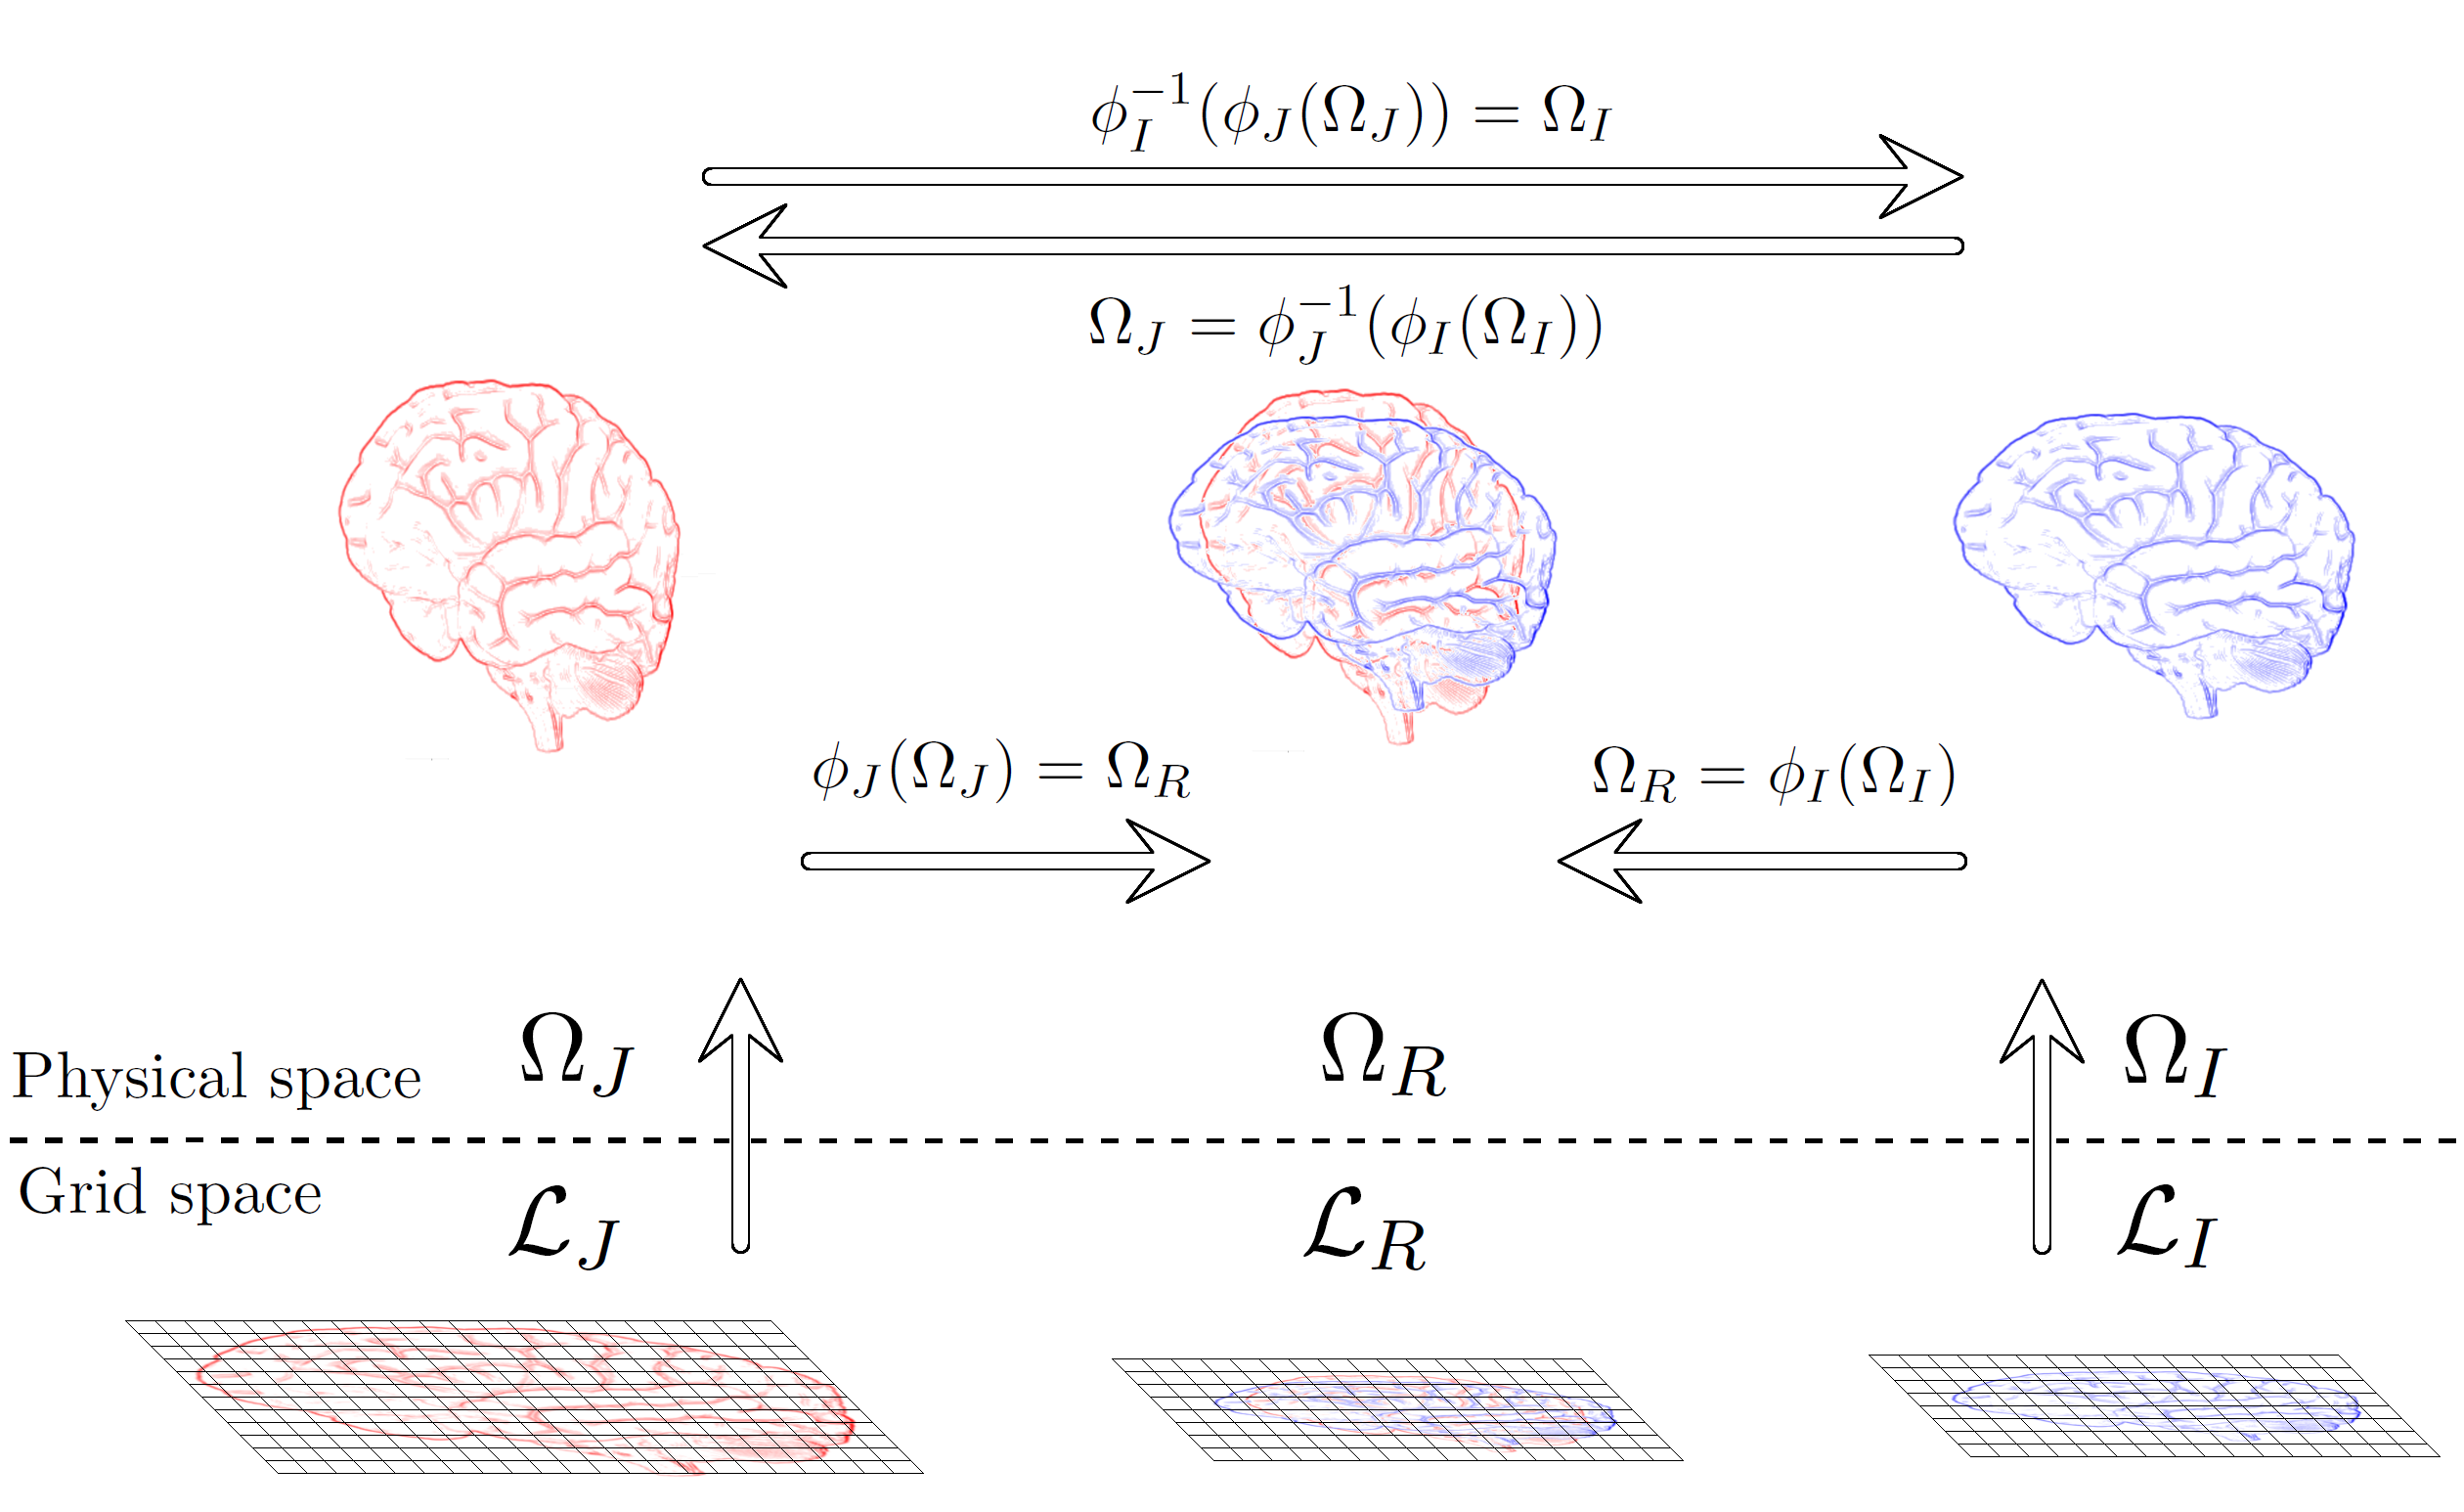
\includegraphics[width=1.0\linewidth]{./images/syn_overview.png}}
\caption{The Greedy SyN algorithm registers two input images by computing two diffeomorphisms that map the input images towards a common reference domain. The final
diffeomorphism is computed by composing the two partial diffeomorphisms.}
\label{fig:syn_overview}
\end{figure}

By defining the warped images \hbox{$\tilde{I}(x) = I(\phi_{I}^{-1}(x))$} and \hbox{$\tilde{J}(x) = J(\phi_{J}^{-1}(x))$} and the hidden random variables \citep{Dempster1977, Li2001}
\begin{equation}\label{eq:hidden_fields}
    \begin{array}{ccc}
        Y(x) &:=& F_{J}\left[\tilde{J}(x)\right]\\[+2mm]
        Z(x) &:=& F_{I}\left[\tilde{I}(x)\right]
    \end{array},x\in\Omega_{R},
\end{equation}
our observation model can be written as
\begin{equation}\label{eq:SyNEM_gom_update}
    \begin{array}{ccccc}
    	Y(x) &=& \tilde{I}(x) &+& \eta_{J}(x)\\
        Z(x) &=& \tilde{J}(x) &+& \eta_{I}(x)
    \end{array}, x\in\Omega_{R}.
\end{equation}
These are precisely two instances of Arce's formulation \citep[see][eq. 1]{Arce-santana2014} in the reference space. The distributions of $Y(x)$ and $Z(x)$ can be written in terms of $\mathbf{I}$ and $\mathbf{J}$ as:
\begin{equation}\label{eq:y_z_i_j_relationship}
    \begin{array}{ccccc}
    	P(Y(x) = i | I, J, \Phi) &=& P(\mathbf{I}=i | \mathbf{J} = J(\phi_{J}^{-1}(x)))\\
        P(Z(x) = j | I, J, \Phi) &=& P(\mathbf{J}=j | \mathbf{I} = I(\phi_{I}^{-1}(x)))\\
    \end{array}, x\in\Omega_{R}.
\end{equation}
Here, we have used the notation $P(\mathbf{I}=i | \mathbf{J} = j)$ instead of \hbox{$P(\mathbf{I}=i | \mathbf{J} = j, I, J, \Phi)$} for simplicity, but it is important to remember that the definition of $P$ depends on $I, J$ and $\Phi$. The conditional expectation and variance of $Y(x)$ given $I, J, \Phi$ can be computed from $P$ as
\begin{equation}\label{eq:expectation_transfer}
    \overline{Y}(x) := \mathbbm{E}\left[\left.Y(x) \right| I, J, \Phi\right] = \mathbbm{E}\left[\left.\mathbf{I} \right| \mathbf{J} = \tilde{J}(x)\right] =
    \int_{\mathbbm{R}} i P(\mathbf{I}=i | \mathbf{J}=\tilde{J}(x)) di
\end{equation}
and
\begin{equation}\label{eq:expectation_variance}
    \sigma_{Y}^{2}(x) := Var\left[\left.Y(x) \right| I, J, \Phi\right] = \int_{\mathbbm{R}} \left(i - \overline{Y}(x)\right)^{2} P(\mathbf{I}=i | \mathbf{J}=\tilde{J}(x)) di.
\end{equation}
Corresponding expressions for $\overline{Z}(x)$ and $\sigma_{Z}^{2}(x)$ are obtained the same way. By performing similar computations as \cite{Arce-santana2014}, we can obtain a symmetric version of the ``EM metric'' to be minimized (named this way since the EM algorithm was used to obtained it), which is the sum of two independent cost functions (see \ref{ap:E_step} for details):
\begin{equation}\label{eq:SyNEM_energy}
    Q(\Phi; \Phi^{(0)}) = Q_{I}(\phi_{I}; \Phi^{(0)}) + Q_{J}(\phi_{J}; \Phi^{(0)})
\end{equation}
given by:
\begin{equation}\label{eq:SyNEM_energy_split}
    \begin{array}{lll}
        Q_{I}(\phi_{I}; \Phi^{(0)}) &=& \sum_{x \in \Omega_{R}} \frac{\left(\overline{Y}(x) - I(\phi_{I}^{-1}(x))\right)^{2}}{2\sigma^{2}_{Y}(x)} + \lambda R(\phi_{I}) \\
        Q_{J}(\phi_{J}; \Phi^{(0)}) &=& \sum_{x \in \Omega_{R}} \frac{\left(\overline{Z}(x) - J(\phi_{J}^{-1}(x))\right)^{2}}{2\sigma^{2}_{Z}(x)} + \lambda R(\phi_{J}) \\
    \end{array}
\end{equation}
where $\Phi^{(0)} = (\phi_{I}^{(0)}, \phi_{J}^{(0)})$ are initial approximations to $\Phi$, and the means and variances of $Y(x)$ and $Z(x)$ are computed using the approximated joint distribution $P(\mathbf{I}, \mathbf{J} | I, J, \Phi^{(0)})$.\\

Notice that $\overline{Y}(x)$ and $\overline{Z}(x)$ are exactly the same optimal transfer functions used in the correlation ratio metric \citep{Roche1998, Roche2000}. Indeed, each of these metrics, derived by \cite{Arce-santana2014}, may be regarded as a generalization of the correlation ratio, which using our notation, is given by \citep[see][eq. 3]{Roche1998}:

\begin{equation}
    CR(I, J, \Phi) = 1 - \frac{Var\left[ \mathbf{I} - \mathbbm{E}\left[ \mathbf{I} | \mathbf{J}\right] \right]}{Var\left[ \mathbf{I} \right]}
\end{equation}
which, in practice, is computed as \citep[see][eq. 4]{Roche1998}:
\begin{equation}
    CR(I, J, \Phi) = 1 - \frac{\frac{1}{|\Omega_{R}|}\sum_{x \in \Omega_{R}} \left(\overline{Y}(x) - I(\phi_{I}^{-1}(x))\right)^{2}}{Var\left[ \mathbf{I} \right]}.
\end{equation}
Therefore, in the special case that all variances $\sigma^{2}_{Y}(x), x\in\Omega_{R}$ are equal, minimizing the EM metric is equivalent to maximizing the correlation ratio metric. The correlation ratio metric arises from an observation model similar to the one presented in \cite{Arce-santana2014}, and extended in this work (eq. \eqref{eq:SyNEM_gom_ref}), but assuming the variance of the noise is constant (see for example eq. 10 in \citep{Roche2000}). However, the EM metric does not make this homoscedasticity assumption, which results in a metric that weighs each squared residual $\left(\overline{Y}(x) - I(\phi_{I}^{-1}(x))\right)^{2}$ using a different factor $\frac{1}{\sigma^{2}_{Y}(x)}$ that measures the uncertainty in the approximation of $\tilde{I}(x)$ by $\overline{Y}(x)$.\\

Functionals $Q_{I}, Q_{J}$ can be efficiently minimized following Vercauteren's analysis of the \textit{diffeomorphic demons} algorithm \citep{Vercauteren2009} as follows.
Let's choose the regularization function $R(\cdot) = ||\nabla \cdot||^{2}$. Starting from the initial transform $\phi^{(0)}_{J}$, we wish to find a small update displacement field $\mathbf{u}$, which minimizes:
\begin{equation}\label{eq:vercauteren_cost}
    \sum_{x \in \Omega_{R}} \frac{\left(\overline{Z}(x) - \tilde{J}(x + \mathbf{u}(x))\right)^{2}}{\sigma^{2}_{Z}(x)} + \lambda ||\nabla \mathbf{u}||^{2}.
\end{equation}

By introducing an auxiliary deformation field $\mathbf{v}$ and a modified energy function
\begin{equation}\label{eq:vercauteren_extended_cost}
    \sum_{x \in \Omega_{R}} \frac{(\overline{Z}(x) - \tilde{J}(x + \mathbf{u}(x)))^{2}}{\sigma^{2}_{Z}(x)} dV + \frac{1}{\tau}||\mathbf{u}-\mathbf{v}||^{2}+\lambda ||\nabla \mathbf{v}||^{2},
\end{equation}
the optimization can be accomplished by alternating two steps. In the first step, we optimize with respect to $\mathbf{u}$ starting with $\mathbf{v} = 0$
\begin{equation}\label{eq:vercauteren_step1}
    \widehat{\mathbf{u}} = \arg\min_{\mathbf{u}}\sum_{x \in \Omega_{R}} \frac{(\overline{Z}(x) - \tilde{J}(x+\mathbf{u}(x)))^{2}}{\sigma^{2}_{Z}(x)} dV + \frac{1}{\tau} ||\mathbf{u}||^{2}.
\end{equation}
We can perform a point-wise minimization by using the first order approximation around the identity
$\tilde{J}(x+\mathbf{u}(x)) \approx \tilde{J}(x) + \nabla \tilde{J}(x)^{T}\mathbf{u}(x)$ and then equating to zero the derivative with respect to $\mathbf{u}(x)$ to obtain:
\begin{equation}\label{eq:euler_lagrange_step1}
    \widehat{\mathbf{u}}(x) = \frac{\overline{Z}(x) - \tilde{J}(x)}{||\nabla \tilde{J}(x)||^{2} + \frac{\sigma_{Z}^{2}(x)}{\tau}}\nabla \tilde{J}(x).
\end{equation}
This expression corresponds to equation (4) in \cite{Vercauteren2009}, but in their work, the factor $\sigma_{Z}^{2}(x)$
is approximated by $\sigma_{Z}(x) \approx |\overline{Z}(x) - \tilde{J}(x)|$ to obtain the traditional {\it demons} step. However, in our case, as in \cite{Arce-santana2014}, we have an explicit and natural estimation of $\sigma^{2}_{Z}(x)$.\\

The second step minimizes eq. \eqref{eq:vercauteren_extended_cost} with respect to $\mathbf{v}$ and keeping fixed the previously obtained displacement field $\mathbf{u}=\widehat{\mathbf{u}}$. The solution of this second sub-problem can be computed by applying a low-pass (smoothing) filter to $\widehat{\mathbf{u}}$. In practice,
this low pass filter is approximated by a Gaussian kernel \citep{Vercauteren2009, Avants2011}.

%To update diffeomorphisms $\phi_{I}, \phi_{J}$ we need to take into consideration that we used their inverses to map images $I, J$ to the reference space. A direct expansion of
%$\tilde{I} \circ \psi$ yields $\phi_{I}^{-1} \leftarrow \phi_{I}^{-1} \circ \psi$, taking its inverse yields $\phi_{I} \leftarrow \psi^{-1} \circ \phi_{I}$, where
%$\psi^{-1} = Id - \mathbf{u}$ for a small displacement field $\mathbf{u}$. We adopted this strategy rather than directly updating the inverses so that the resulting algorithm
%(Alg. \ref{alg:SyNEM})is equivalent to the Greedy SyN algorithm previously described (Alg. \ref{alg:Greedy_SyN}), which has been extensively tested by the neuroimaging
%community.

\subsection{Expected Cross-Correlation}\label{sec:syn_ecc}
The main drawback of using a point-wise metric like SSD, the EM metric previously described, or Mutual Information, is that they are unable to capture important features from the voxels' neighborhood like gradients and texture. Being point-wise, any permutation of the voxels' positions results in exactly the same measured similarity (provided the same permutation is applied to both, the moving and fixed images). This makes point-wise metrics more susceptible to noise and image artifacts such as the bias field in MRI. By considering small windows $W_{y}$ around each voxel $y\in\Omega_{R}$, the normalized Cross Correlation metric (CC), takes advantage of more complex local information, resulting in a more robust metric:
\begin{equation}
    CC(y;\tilde{I}, \tilde{J}) = \frac{\left[\sum_{z\in W_{y}} \left(\tilde{I}(z) - \mu_{y}\right)\left(\tilde{J}(z) - \nu_{y}\right)\right]^{2}}
    {\left[\sum_{z \in W_{y}}\left(\tilde{I}(z) - \mu_{y}\right)^{2}\right] \left[\sum_{z \in W_{y}}\left(\tilde{J}(z) - \nu_{y}\right)^{2}\right]}
\end{equation}
where
\begin{equation}
    \begin{array}{lll}
        \mu_{y} &=& \frac{1}{|W_{y}|}\sum_{z \in W_{y}}\tilde{I}(z)\\
        \nu_{y} &=& \frac{1}{|W_{y}|}\sum_{z \in W_{y}}\tilde{J}(z)\\
    \end{array}.
\end{equation}

The EM formulation belongs to the class of multi-modal image registration methods that reduce the multi-modal problem to a mono-modal one \citep{Sotiras2013}. One of the advantages of this class of methods is that it is relatively easy to extend other mono-modal metrics to the multi-modal case using the same ideas. In particular, we can extend the CC metric for multi-modal images by defining the {\it Expected Cross Correlation} metric as:
\begin{equation}\label{eq:ecc_metric}
    ECC(y;\tilde{I}, \tilde{J}) = CC(y; \overline{Y}, \tilde{I}) + CC(y; \overline{Z}, \tilde{J})
\end{equation}

The first term measures the similarity between $\overline{Y}$ and $\tilde{I}$ (corresponding to a similarity measure in the modality of $I$), while the second term measures the
similarity between $\overline{Z}$ and $\tilde{J}$ (corresponding to a similarity measure in the modality of $J$). The resulting algorithm (see \ref{ap:Algorithms}, alg. \ref{alg:SyNECC}) is, therefore, a combination of the Greedy-SyN algorithm (\ref{alg:Greedy_SyN}) and the SyN-EM algorithm (see \ref{ap:CC_gradient} for details on
computing the gradients).


\subsection{Experiments}
Validation is one of the most challenging aspects of developing image registration algorithms. In order to rigorously evaluate the performance of non-linear
image registration algorithms, we would require a ground-truth consisting of true correspondences between voxels of realistic pairs of images. Since such a ground-truth data are not currently available, researchers resort to surrogates that indirectly measure the quality of their algorithms. For brain MRI registration, for instance, one of the most accepted surrogate measures, is based on the overlap of localized anatomical areas of registered images: ideally, corresponding anatomical areas of perfectly registered images should perfectly overlap. Even a perfect registration algorithm is unlikely to achieve such an ambitious goal, though, since anatomical areas are usually defined manually by an expert, which is by no means a perfect process and the annotations may vary even between different experts. Despite this limitation, it has been shown that among the alternative surrogate measures usually employed, overlap scores of localized anatomical areas is the one that better distinguish reasonable from inaccurate registrations \citep{Rohlfing2012} and it has been employed in the most rigorous evaluations of registration algorithms \citep{Klein2009, Klein2010, Rohlfing2012}. In our experiments, we employ the publicly available Internet Brain Segmentation Repository (IBSR) database consisting of 18 manually annotated T1 brain MRI volumes. Our algorithms are publicly available from the Dipy non-linear registration module \citep{Garyfallidis2014}.\\ 

The methods under evaluation in this section are: 1) SyN with the Normalized Cross Correlation metric \citep{Avants2008, Avants2011}, denoted ``SyN-CC'', 2) SyN with the Mutual Information metric \citep{Mattes2003, Avants2011}, denoted ``SyN-MI'', available in the ANTs software package, 3) the SyN-EM algorithm (see \ref{ap:Algorithms}, alg. \ref{alg:SyNEM}) proposed in section \ref{sec:syn_em}, and 4) the SyN-ECC algorithm (see \ref{ap:Algorithms}, alg. \ref{alg:SyNECC}) proposed in section \ref{sec:syn_ecc}. 
\section{Experiments}
We compared the accuracy of four matching functionals driving the SyN transformation model: CC, MI, EM and ECC. We selected the CC functional because its robustness and accuracy for mono-modal registration have been demonstrated in large scale comparative studies \citep{Klein2009, Klein2010, Rohlfing2012} (it would be desirable to reach similar performance in the multi-modal case), we would like to quantify how large is its drop in accuracy for multi-modal images. MI \citep{Maes1997, Mattes2003} may be considered the functional of choice for multi-modal registration, it is expected that any new developed functional yields results at least as good as MI. The EM functional \cite{Arce-santana2014} is, to the best of our knowledge, the most recent proposal for multi-modal registration based on the assumption of a functional relationship between image modalities. It introduces a measure of uncertainty for each intensity, which may help to alleviate the effects of non-stationary relationships between image intensities. We implemented the EM functional to drive the SyN transformation model and extended it to make it symmetric (to estimate both transfer functions instead of only one), in our experiments, these modifications performed significantly better than the basic functional (non-symmetric, and using an elastic transformation model) proposed by Arce {\it et al.}\cite{Arce-santana2014}. Both MI and EM are voxel-wise functionals (i.e. it compares pairs of single voxels), while CC and ECC are computed from local rectangular windows.

\subsection{Mono-modal registration}
Although our matching functional was designed for multi-modal image registration, it is important to first verify that the quality of the algorithms is reasonable for mono-modal registration. Figure \ref{fig:mono_graph_seg} show the average overlap score for each of 31 manually annotated anatomical regions from the IBSR database. Note that the Jaccard indices obtained with CC (i.e. ANTS) are higher than reported by Rohlfing \cite{Rohlfing2012}. In his experiments, he used three resolutions with a maximum of 10, 10 and 5 iterations only. Here, we set a maximum of 100, 100 and 25 iterations, leaving the rest of the parameters unchanged (the same for all functionals). We can see that SyN with the EM metric is very competitive, but still not as good as CC. This may be explained by the fact that CC uses a window centered at each voxel for computing the similarity, while the EM is voxelwise. This behavior can also be observed from the results of SyN with Mutual Information (MI), which is also voxel-wise and very competitve but not as good as CC. By considering neighborhoods of the same size, the performance of ECC is practically the same as CC. Table \ref{tab:monomodal_results_segTri_fill} shows the overlap scores over tissue types (white matter, gray matter and cerebrospinal fluid), instead of anatomical areas.
%Table \ref{tab:monomodal_results_seg} and
%% Table generated by Excel2LaTeX from sheet 'SyNEM-Monomodal-Large'
\begin{table}[p]
\begin{adjustwidth}{-0.75cm}{}
  {\centering
    \small
    \begin{tabular}{lcccc}
    \toprule
    \textbf{}& \textbf{SyN-EM} & \textbf{SyN-ECC} & \textbf{SyN-CC} & \textbf{SyN-MI} \\
    \midrule
    \textbf{Brain-Stem} & 0.786 & \textbf{0.816} & 0.812 & 0.804 \\
    \textbf{Right-Cerebellum-Cortex} & 0.736 & \textbf{0.815} & 0.813 & 0.771 \\
    \textbf{Left-Cerebellum-Cortex} & 0.739 & \textbf{0.811} & 0.808 & 0.766 \\
    \textbf{Right-Thalamus-Proper} & 0.714 & 0.766 & \textbf{0.772} & 0.745 \\
    \textbf{Left-Thalamus-Proper} & 0.727 & 0.763 & \textbf{0.767} & 0.748 \\
    \textbf{Right-Putamen} & 0.681 & 0.748 & \textbf{0.751} & 0.712 \\
    \textbf{Left-Putamen} & 0.699 & 0.744 & \textbf{0.744} & 0.721 \\
    \textbf{Left-Cerebral-Cortex} & 0.724 & \textbf{0.739} & 0.733 & 0.687 \\
    \textbf{Right-Cerebral-Cortex} & 0.719 & \textbf{0.739} & 0.731 & 0.683 \\
    \textbf{Right-Cerebral-White-Matter} & 0.702 & \textbf{0.733} & 0.720 & 0.645 \\
    \textbf{Left-Cerebral-White-Matter} & 0.705 & \textbf{0.732} & 0.721 & 0.646 \\
    \textbf{Left-Lateral-Ventricle} & 0.731 & 0.727 & \textbf{0.732} & 0.718 \\
    \textbf{Right-Lateral-Ventricle} & 0.709 & 0.714 & \textbf{0.717} & 0.699 \\
    \textbf{Right-Cerebellum-White-Matter} & 0.576 & \textbf{0.701} & 0.691 & 0.608 \\
    \textbf{Left-Cerebellum-White-Matter} & 0.581 & \textbf{0.701} & 0.693 & 0.611 \\
    \textbf{Left-Caudate} & 0.645 & \textbf{0.671} & 0.665 & 0.666 \\
    \textbf{Right-Caudate} & 0.620 & \textbf{0.655} & 0.647 & 0.651 \\
    \textbf{Right-VentralDC} & 0.612 & 0.651 & \textbf{0.652} & 0.628 \\
    \textbf{Left-VentralDC} & 0.622 & \textbf{0.651} & 0.650 & 0.631 \\
    \textbf{Right-Pallidum} & 0.498 & \textbf{0.622} & 0.620 & 0.582 \\
    \textbf{Right-Hippocampus} & 0.572 & \textbf{0.621} & 0.620 & 0.575 \\
    \textbf{Left-Pallidum} & 0.524 & \textbf{0.615} & 0.614 & 0.583 \\
    \textbf{Left-Hippocampus} & 0.574 & \textbf{0.610} & 0.609 & 0.564 \\
    \textbf{4th-Ventricle} & 0.551 & 0.606 & \textbf{0.608} & 0.574 \\
    \textbf{3rd-Ventricle} & 0.527 & 0.544 & \textbf{0.547} & 0.515 \\
    \textbf{Left-Amygdala} & 0.444 & 0.519 & \textbf{0.519} & 0.484 \\
    \textbf{Right-Amygdala} & 0.411 & 0.513 & \textbf{0.514} & 0.458 \\
    \textbf{Left-Accumbens-area} & 0.451 & 0.500 & \textbf{0.500} & 0.462 \\
    \textbf{Right-Accumbens-area} & 0.433 & 0.490 & \textbf{0.490} & 0.443 \\
    \textbf{Right-Inf-Lat-Vent} & 0.177 & 0.230 & \textbf{0.232} & 0.162 \\
    \textbf{Left-Inf-Lat-Vent} & 0.190 & 0.228 & \textbf{0.233} & 0.167 \\
    \hline
    \textbf{Average (std.)} & 0.593 (0.148) & 0.644 (0.142) & 0.643 (0.140) & 0.603 (0.149) \\
    \textbf{Rank-1 count} & 0 & 16 & 15 & 0 \\
    \textbf{Rank-2 count} & 1 & 14 & 14 & 2 \\
    \textbf{Rank-3 count} & 9 & 1 & 2 & 19 \\
    \bottomrule
    \end{tabular}}%
    \caption{Comparison of the registration performance (measured by the Jaccard index over 31 anatomical regions) of the Greedy SyN algorithm with EM, ECC, CC and MI metrics.
The Jaccard indices were averaged over 306 monomodal registrations. Rank-$k$ counts show the number of anatomical regions for which each
method ranked $k$ among the four methods under comparison. Top performer (rank-1) for each region is highlighted. }
  \label{tab:monomodal_results_seg}%
\end{adjustwidth}
\end{table}%

% Table generated by Excel2LaTeX from sheet 'SyNEM-Monomodal-Large'
\begin{table}[htbp]
  \centering
  {\small
    \begin{tabular}{rrrr}
    \toprule
    \textbf{} & \textbf{SyN-EM} & \textbf{SyN-ECC} & \textbf{SyN-CC} \\
    \midrule
    \textbf{Background} & 0.994 & 0.995 & \textbf{0.995} \\
    \textbf{CSF} & 0.335 & 0.349 & \textbf{0.359} \\
    \textbf{Gray Matter} & 0.740 & \textbf{0.765} & 0.759 \\
    \textbf{White Matter} & 0.703 & \textbf{0.739} & 0.728 \\
    \bottomrule
    \end{tabular}%
    \caption{Comparison of the registration performance (measured by the Jaccard index over Background, CSF, GM and WM)of the Greedy SyN algorithm with EM, ECC and CC metrics. The Jaccard
indices were averaged over 306 monomodal registrations. Top performer for each region is highlighted.}
  \label{tab:monomodal_results_segTri_fill}}%
\end{table}%


\begin{figure*}[t!]
\centering
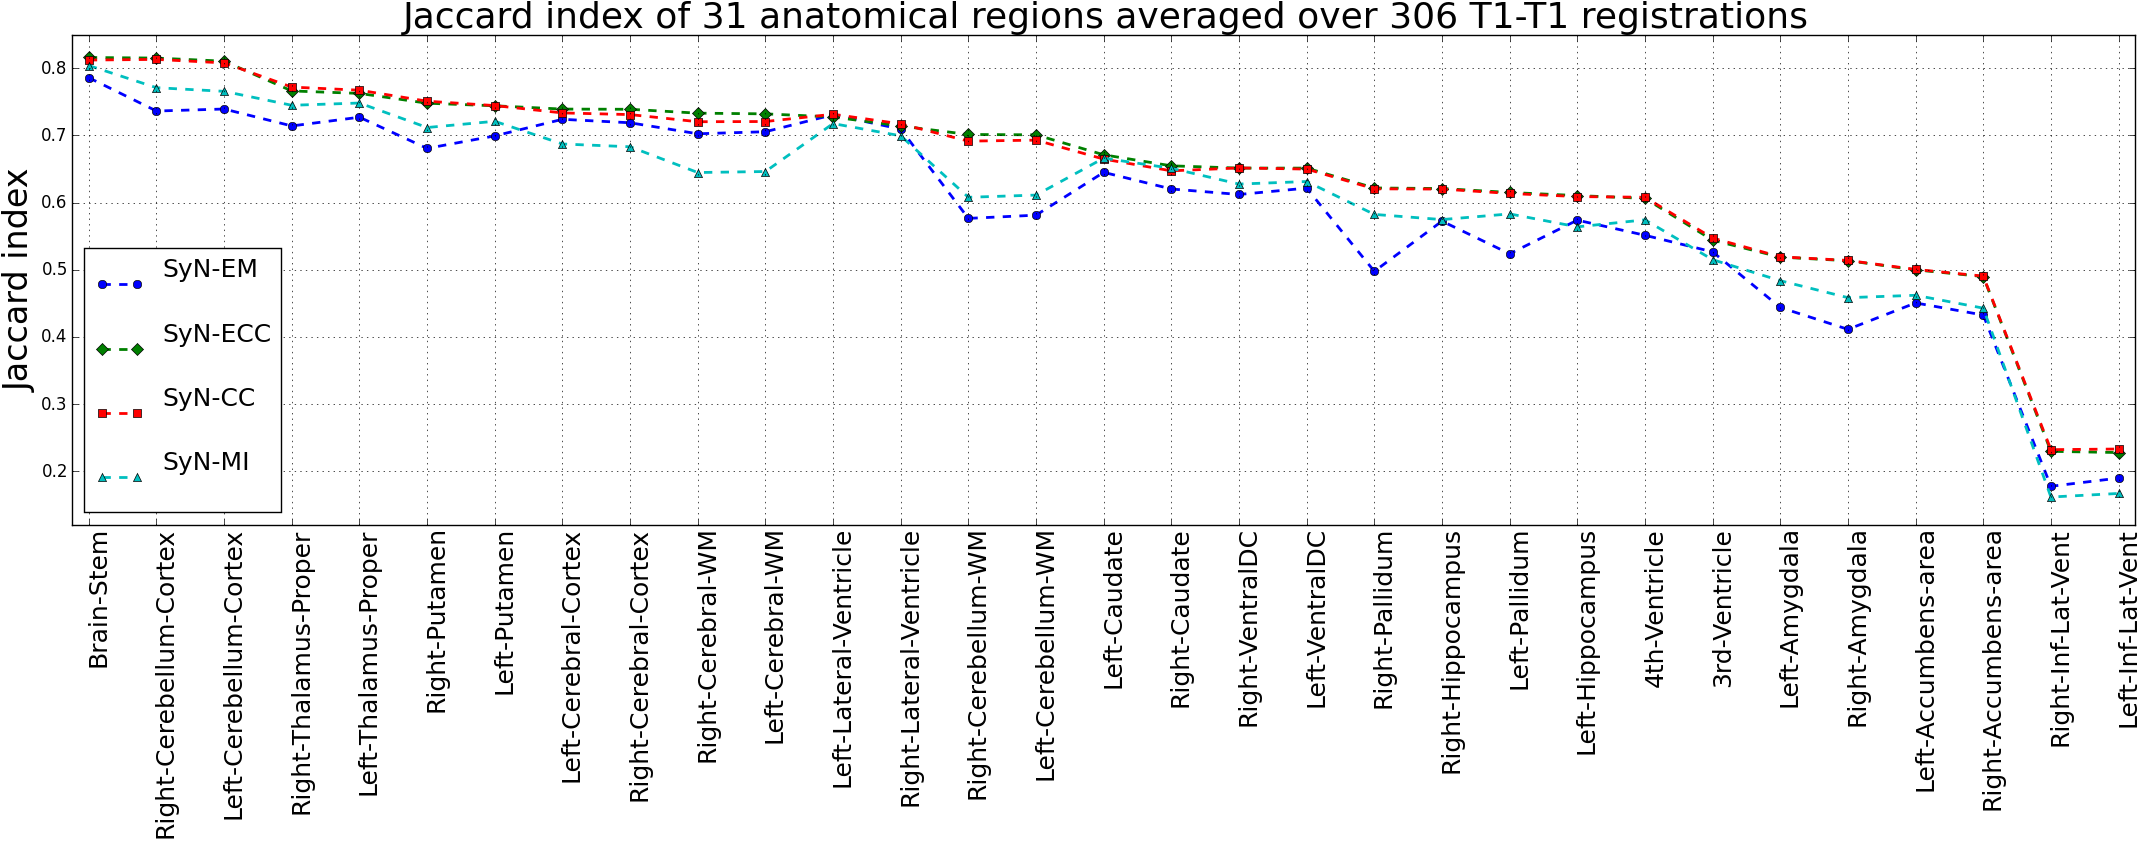
\includegraphics[width=1.0\linewidth]{./images/mono_lines_seg.png}\\
\caption{{\small Comparison of the registration performance (measured by the Jaccard index over 31 anatomical regions) of the Greedy SyN algorithm with EM, ECC, CC and MI metrics. The Jaccard indices were averaged over 306 monomodal registrations.}}
\label{fig:mono_graph_seg}
\end{figure*}

\subsection{Multi-modal registration}\label{sec:multimodal_results}

Unfortunately, to the best of our knowledge, there are no manually annotated multi-modal data publicly available to evaluate the registration performance quantitatively. Instead, we generated synthetic T2 images for all IBSR T1 images as follows. We first register the Brainweb T1 template (which plays the role of moving image) towards each IBSR T1 image (which play the role of fixed images) using ANTs with the CC metric (a mono-modal registration problem). Then we applied the resulting deformation field to the Brainweb T2 template. The transfer function from the real T1 image to the warped T2 template is computed as the average T2 intensity associated to each T1 intensity. The computed transfer function is then applied to the real IBSR T1 image obtaining a ``perfectly aligned'' realistic synthetic T2 image for each IBSR volume, therefore the annotations remain exactly the same as the T1 counterparts and we are able to compute the overlap scores as before. Note that the number of registrations we need to perform is now 612 because we can use the T2 modality either as the moving or the fixed image. Figure \ref{fig:multi_seg} shows results similar to Figure \ref{fig:mono_graph_seg} but this time averaged over 612 multimodal registrations. Note how the performance of the CC metric strongly drops while EM, ECC and MI are less affected by the change of modality. Table \ref{tab:multimodal_results_segTri_fill} shows the overlap scores of tissue types, where the same behavior can be observed.\\
%Table \ref{tab:monomodal_results_seg} and
%Table \ref{tab:multimodal_results_seg} and
%\begin{figure}[H]
%\centering
%    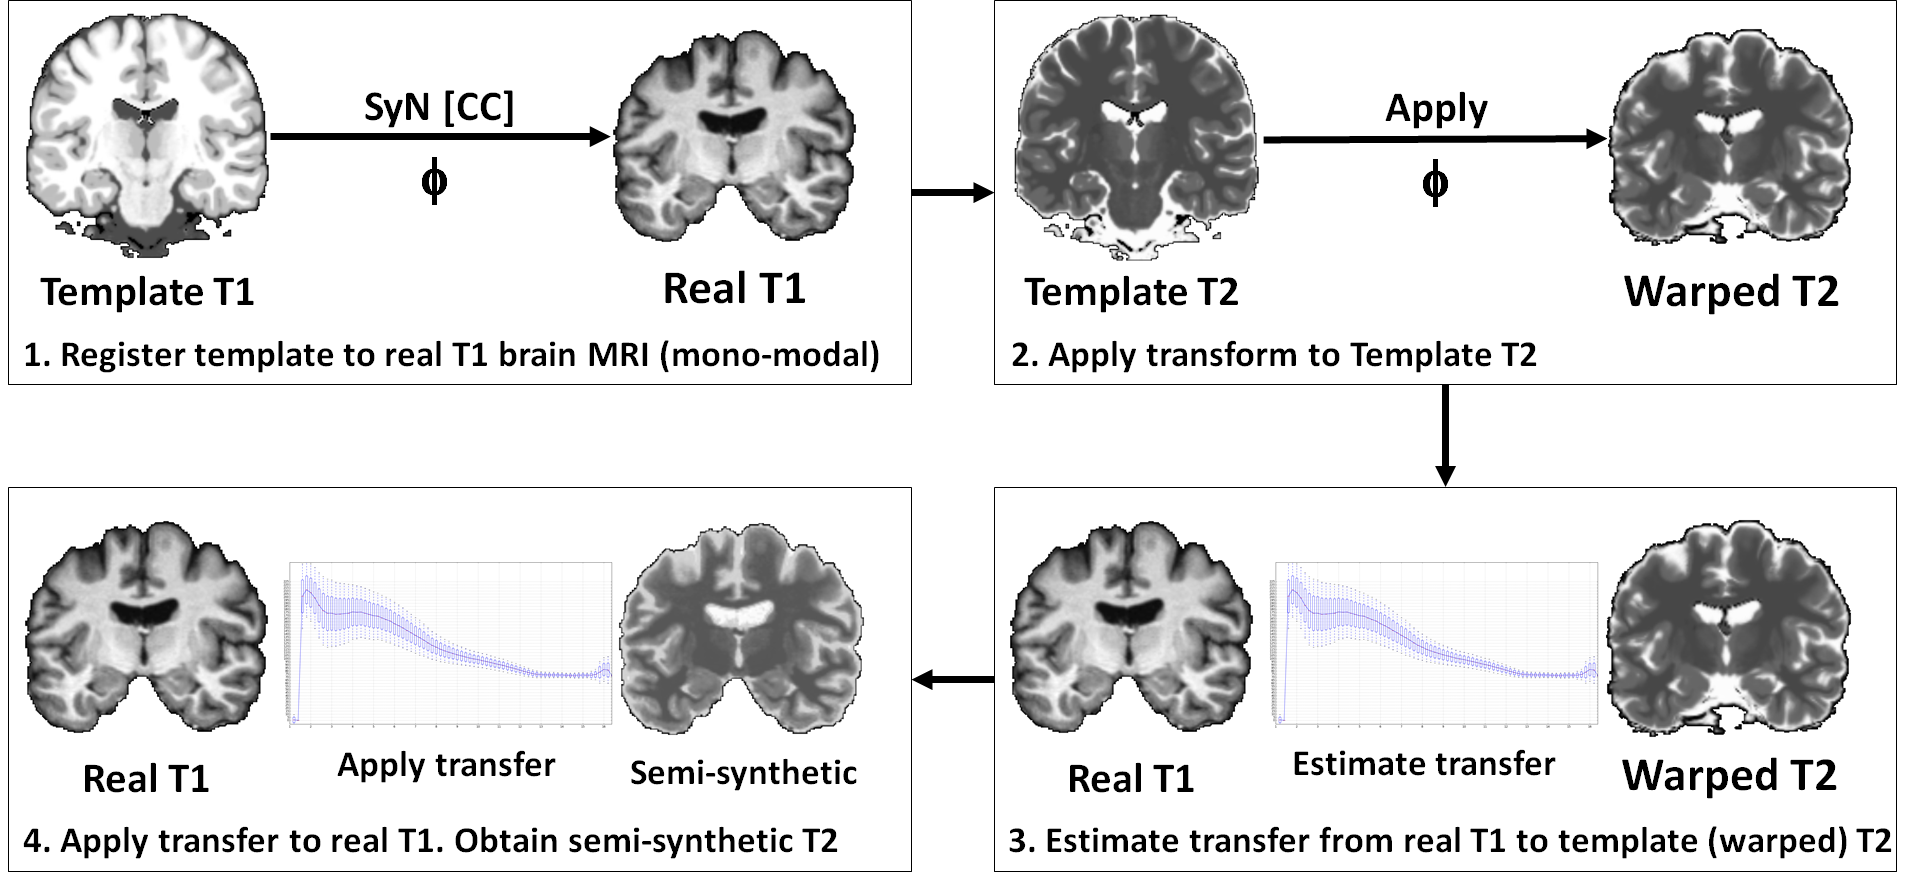
\includegraphics[width=\linewidth]{./images/semi_synthetic_image_creation.png}
%    \caption{{\small Semi-synthetic, manually annotated images for quantitative evaluation of multi-modal non-linear image registration algorithms.}}
%\label{fig:semi_synthetic_image_creation}
%\end{figure}

The Brainweb template also provides us with a simulation of a proton density (PD) image for the same brain anatomy. This allows us to repeat the procedure described above for each pair of three modalities, T1, T2 and PD, which results in 3 mono-modal and 3 multi-modal registration experiments. For the sake of brevity, Figure \ref{fig:all_pairs_boxplots} depicts a summary of the results obtained over all pairs of modalities. For each pair of registered images, we compute the average Jaccard index of all anatomical regions. Each boxplot in Figure \ref{fig:all_pairs_boxplots} corresponds to the set of all 306 (mono-modal) or 612 (multi-modal) average scores for that particular method and that particular pair of modalities. We can observe that the CC metric performs very well for all mono-modal experiments (diagonal graphs), but it is severely affected in the multi-modal case (off-diagonal graphs). The ECC metric performs practically the same as CC in the mono-modal case, but is less affected in the multi-modal case. By measuring the similarity of local windows instead of individual voxels, the ECC metric outperforms the EM and MI metrics in all cases.

%% Table generated by Excel2LaTeX from sheet 'SyNEM-Multi-Large'
\begin{table}[htbp]
  \centering
  {\small
    \begin{tabular}{rrrr}
    \toprule
          & \textbf{SyN-ECC} & \textbf{SyN-EM} & \textbf{SyN-CC} \\
    \midrule
    \textbf{Right-Thalamus-Proper:} & \textbf{0.758} & 0.716 & 0.756 \\
    \textbf{Left-Thalamus-Proper:} & \textbf{0.754} & 0.727 & 0.752 \\
    \textbf{Left-Lateral-Ventricle:} & 0.709 & 0.706 & \textbf{0.733} \\
    \textbf{Right-Lateral-Ventricle:} & 0.696 & 0.687 & \textbf{0.718} \\
    \textbf{Left-Putamen:} & \textbf{0.740} & 0.699 & 0.683 \\
    \textbf{Right-Putamen:} & \textbf{0.742} & 0.684 & 0.676 \\
    \textbf{Brain-Stem:} & \textbf{0.790} & 0.786 & 0.663 \\
    \textbf{Left-Cerebellum-Cortex:} & \textbf{0.765} & 0.729 & 0.649 \\
    \textbf{Right-Cerebellum-Cortex:} & \textbf{0.769} & 0.729 & 0.645 \\
    \textbf{Left-Caudate:} & \textbf{0.652} & 0.628 & 0.637 \\
    \textbf{Right-Caudate:} & \textbf{0.636} & 0.606 & 0.618 \\
    \textbf{Right-Cerebral-White-Matter:} & \textbf{0.723} & 0.683 & 0.571 \\
    \textbf{Left-Cerebral-White-Matter:} & \textbf{0.722} & 0.685 & 0.570 \\
    \textbf{Left-Cerebral-Cortex:} & \textbf{0.700} & 0.699 & 0.558 \\
    \textbf{Right-Cerebral-Cortex:} & \textbf{0.697} & 0.694 & 0.548 \\
    \textbf{4th-Ventricle:} & \textbf{0.583} & 0.546 & 0.543 \\
    \textbf{Right-Hippocampus:} & \textbf{0.610} & 0.570 & 0.503 \\
    \textbf{Right-VentralDC:} & \textbf{0.642} & 0.616 & 0.499 \\
    \textbf{Right-Pallidum:} & \textbf{0.606} & 0.528 & 0.499 \\
    \textbf{Left-Pallidum:} & \textbf{0.602} & 0.545 & 0.495 \\
    \textbf{3rd-Ventricle:} & \textbf{0.517} & 0.511 & 0.492 \\
    \textbf{Left-VentralDC:} & \textbf{0.640} & 0.622 & 0.491 \\
    \textbf{Left-Hippocampus:} & \textbf{0.600} & 0.567 & 0.488 \\
    \textbf{Left-Cerebellum-White-Matter:} & \textbf{0.688} & 0.582 & 0.485 \\
    \textbf{Right-Cerebellum-White-Matter:} & \textbf{0.690} & 0.579 & 0.476 \\
    \textbf{Left-Amygdala:} & \textbf{0.505} & 0.447 & 0.360 \\
    \textbf{Right-Amygdala:} & \textbf{0.497} & 0.415 & 0.339 \\
    \textbf{Right-Accumbens-area:} & \textbf{0.483} & 0.433 & 0.339 \\
    \textbf{Left-Accumbens-area:} & \textbf{0.494} & 0.448 & 0.338 \\
    \textbf{Left-Inf-Lat-Vent:} & \textbf{0.219} & 0.178 & 0.194 \\
    \textbf{Right-Inf-Lat-Vent:} & \textbf{0.219} & 0.164 & 0.178 \\
    \bottomrule
    \end{tabular}}%
    \caption{Comparison of the registration performance (measured by the Jaccard index over 31 anatomical regions) of the Greedy SyN algorithm with EM, ECC and CC metrics. The Jaccard
indices were averaged over 612 multimodal registrations. Top performer for each region is highlighted.}
  \label{tab:multimodal_results_seg}%
\end{table}%

% Table generated by Excel2LaTeX from sheet 'SyNEM-Multi-Large'
\begin{table}[htbp]
  \centering
  {\small
    \begin{tabular}{ccccc}
    \toprule
          & \textbf{SyN-EM} & \textbf{SyN-ECC} & \textbf{SyN-CC} & \textbf{SyN-MI} \\
    \midrule
    \textbf{Background} & 0.993 & 0.995 & 0.990 & \textbf{0.995} \\
    \textbf{CSF} & 0.275 & \textbf{0.335} & 0.157 & 0.325 \\
    \textbf{Gray Matter} & 0.718 & \textbf{0.742} & 0.597 & 0.691 \\
    \textbf{White Matter} & 0.685 & \textbf{0.718} & 0.572 & 0.622 \\
    \bottomrule
    \end{tabular}}%
  \caption{Comparison of the registration performance (measured by the Jaccard index over Background, CSF, GM and WM)of the Greedy SyN algorithm with EM, ECC, CC and MI metrics.
The Jaccard indices were averaged over 612 multimodal registrations. Top performer for each region is highlighted.}
  \label{tab:multimodal_results_segTri_fill}%
\end{table}%


\begin{figure*}[t!]
\centering
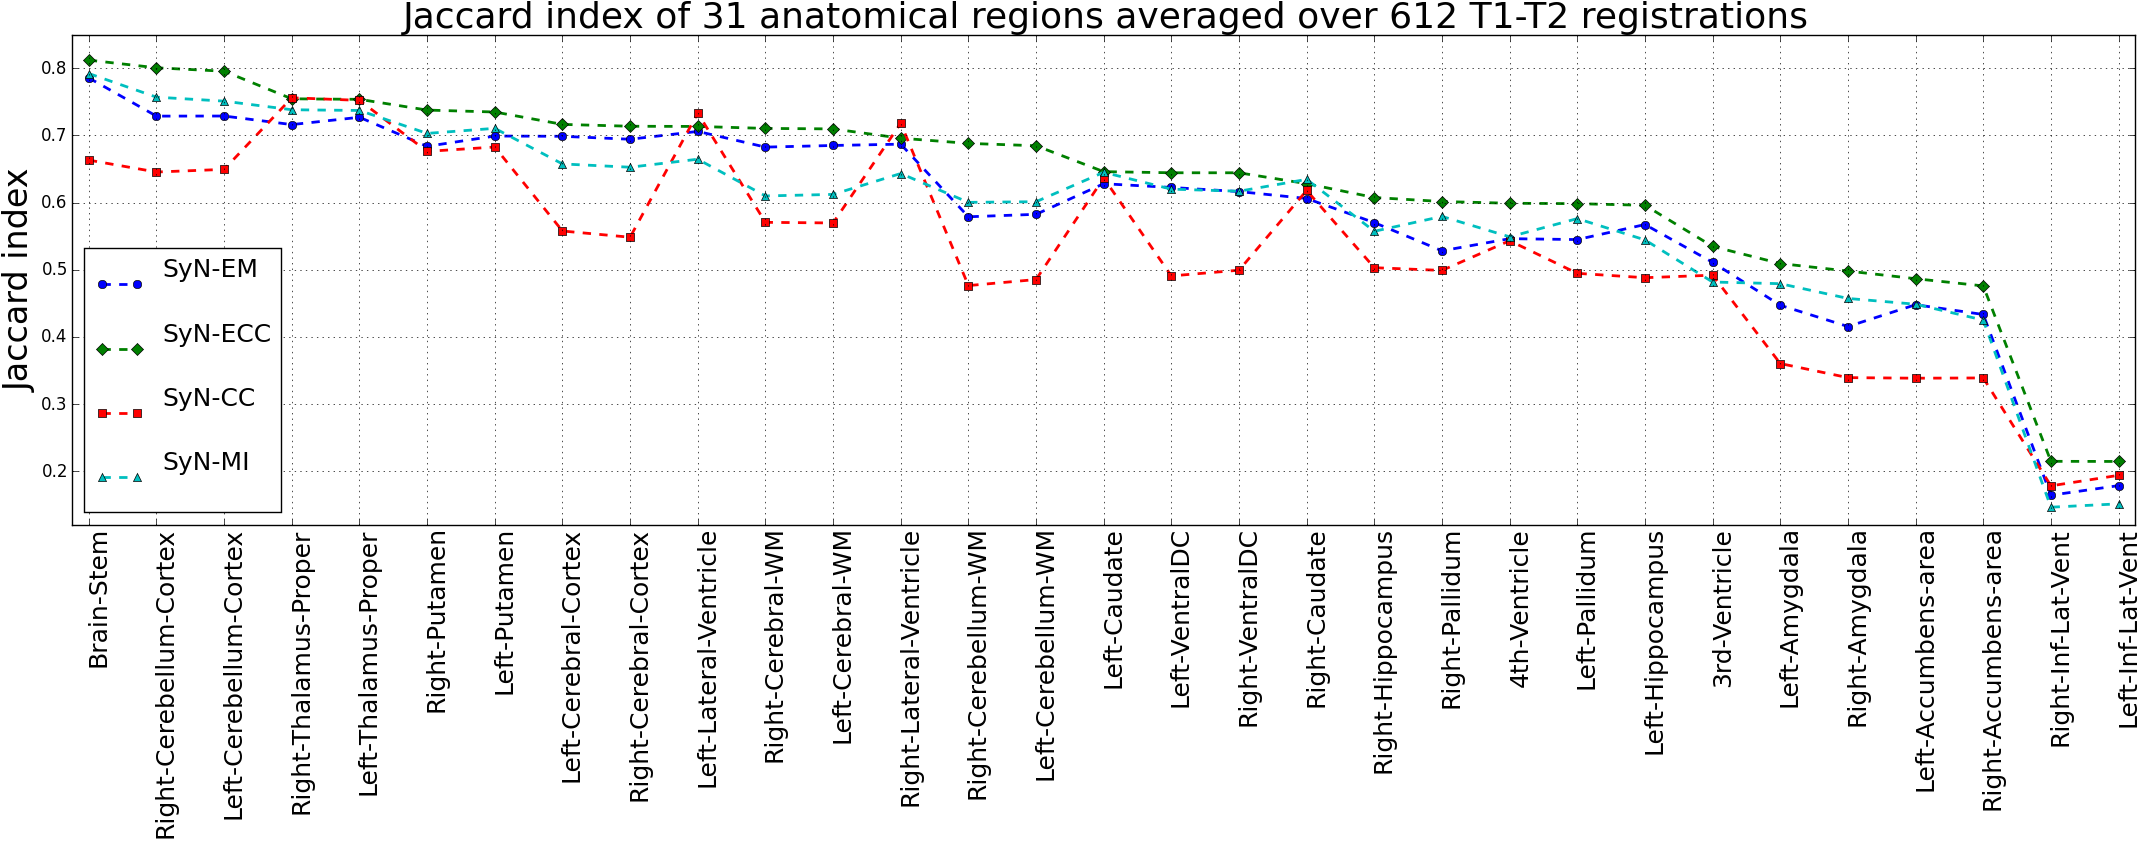
\includegraphics[width=1.0\linewidth]{./images/multi_lines_seg.png}\\
\caption{{\small Comparison of the registration performance (measured by the Jaccard index over 31 anatomical regions) of the Greedy SyN algorithm with EM, ECC, CC and MI metrics. The Jaccard indices were averaged over 612 multimodal registrations.}}
\label{fig:multi_seg}
\end{figure*}

\begin{figure}[t!]
\centering
    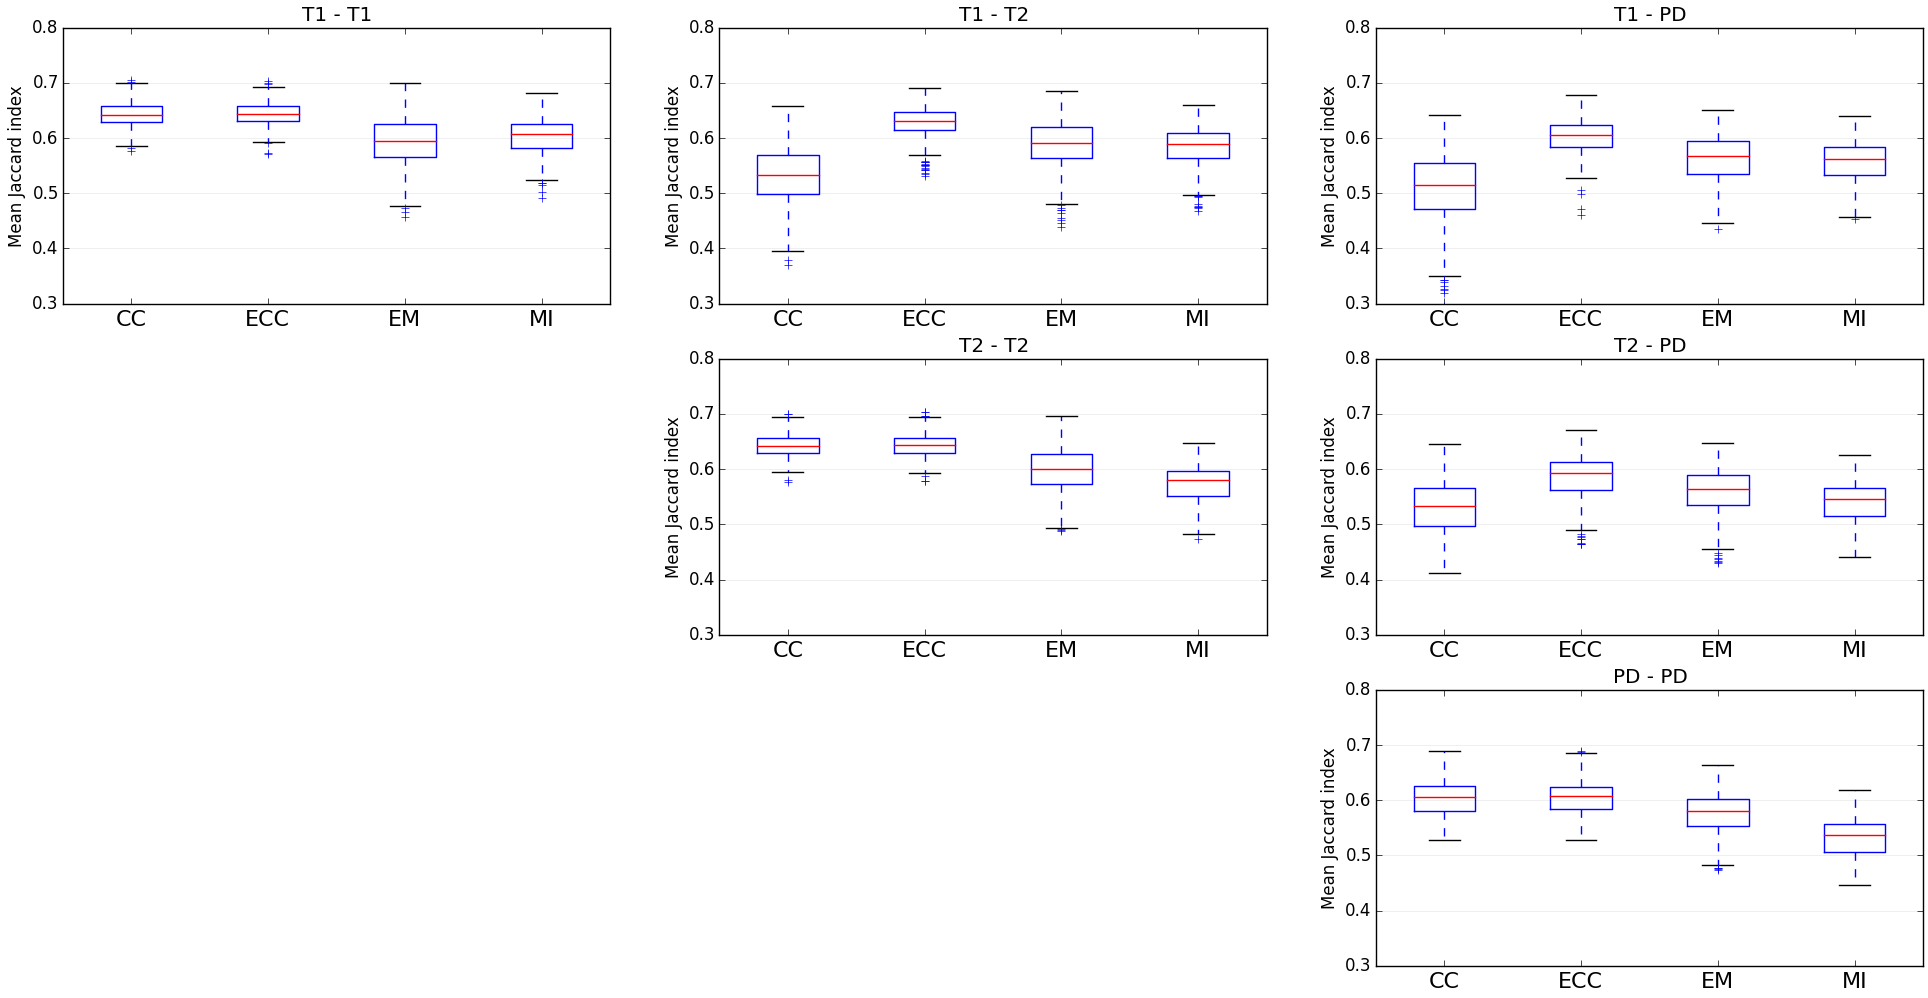
\includegraphics[width=\linewidth]{./images/all_modality_pairs_boxplots.png}
    \caption{{\small Distributions of average Jaccard indices for all pairs of available modalities (T1, T2 and PD). For each pair of registrations, we compute the average Jaccard index of all anatomical regions. The boxplots show the distribution of all such average overlap scores.}}
\label{fig:all_pairs_boxplots}
\end{figure}

\subsection{$B_{0}$-T1 registration}
Quantitative results shown in previous section indicate that ECC and MI perform best for multi-modal registration. Fig. \ref{fig:comparison_B0_T1_coregistration} depicts a a $B_{0}$-T1 registration result obtained using using ECC and MI. We can see from the level curves that the result obtained with ECC matches better the local structure of the T1. This behavior is explained by the fact that the ECC functional is computed over pairs of local windows rather than single voxel pairs.\\
%\begin{figure}[p]
%\centering
%    \subfloat[Example $B_{0}$-T1 registration result using SyN with %ECC.]{\label{fig:epicor_b0up_ecc}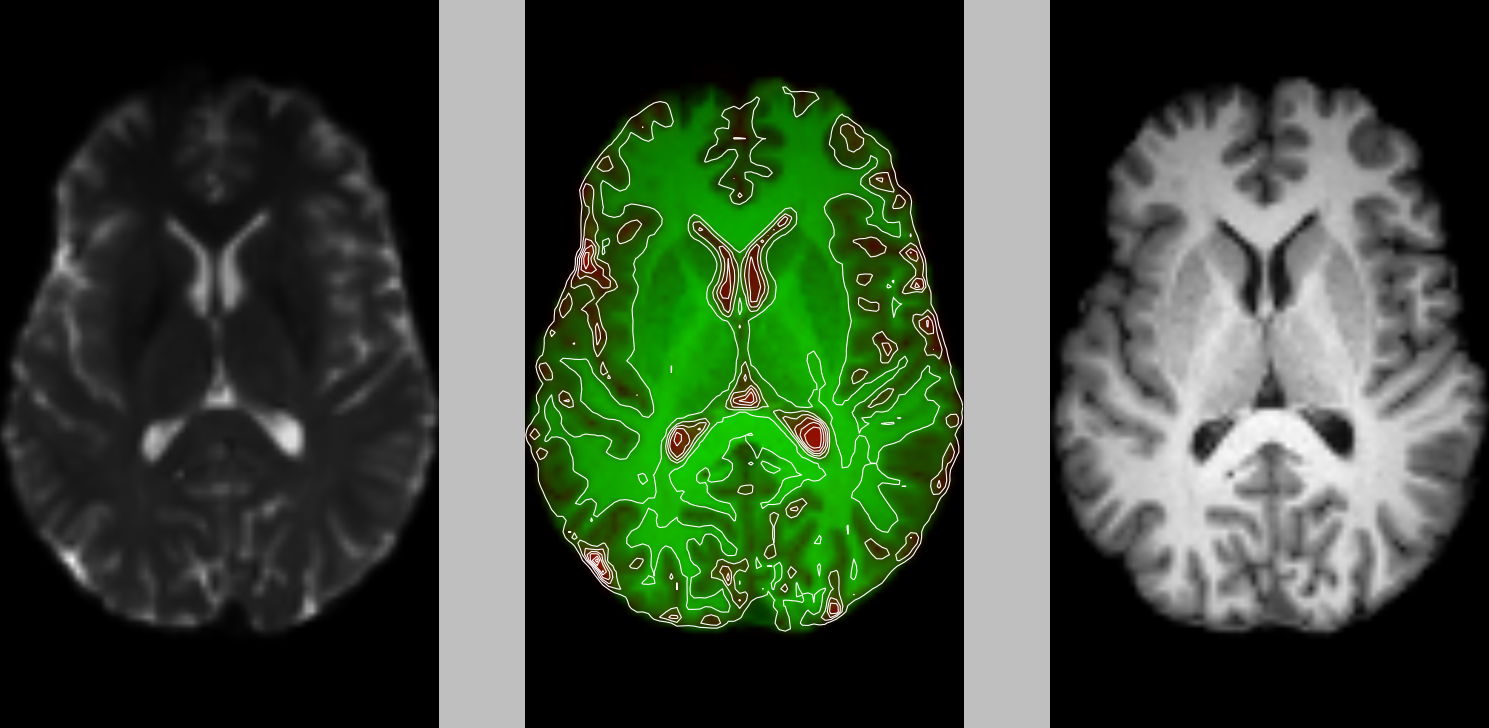
\includegraphics[width=1.0\linewidth]{./images/T1B0Result/epicor_b0up_ecc.png}}\\
%    \subfloat[Example $B_{0}$-T1 registration result using SyN with MI.]{\label{fig:epicor_b0up_mi}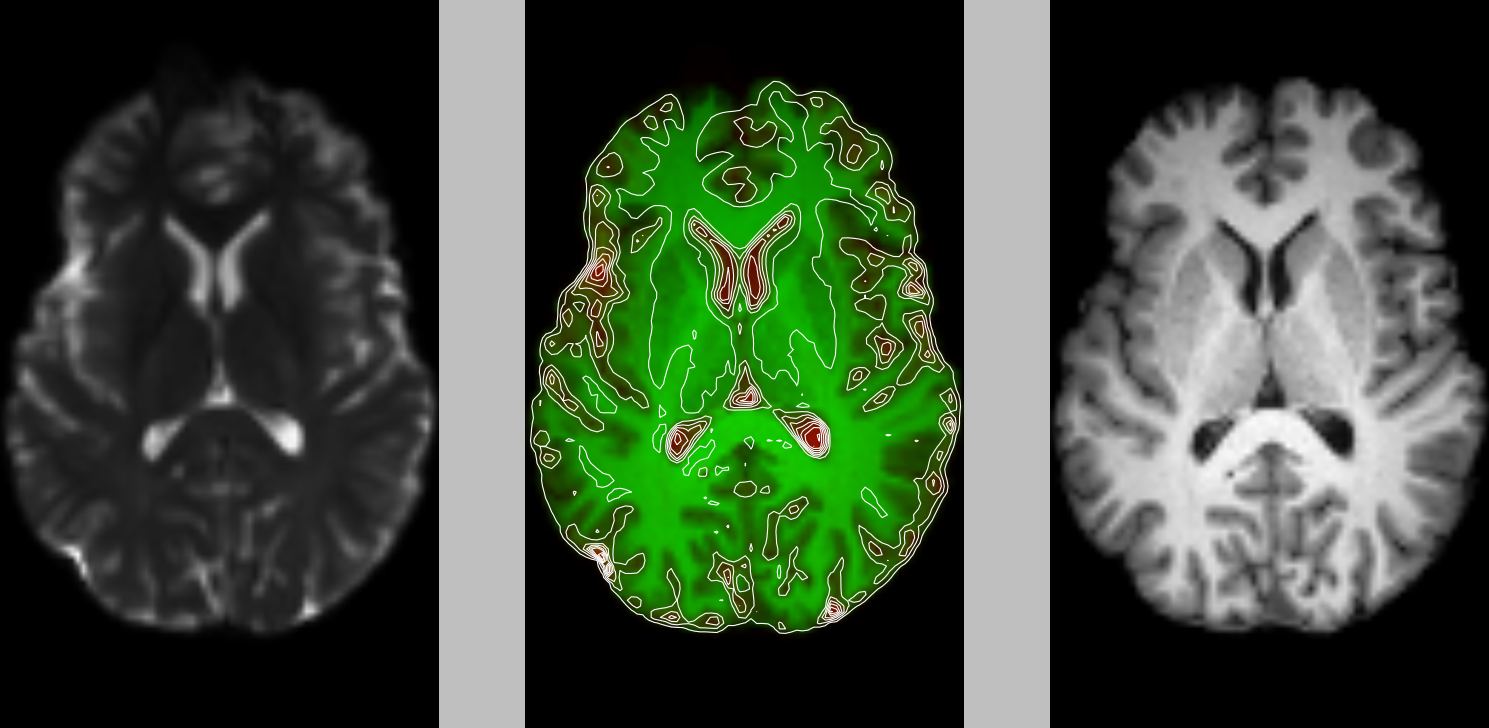
\includegraphics[width=1.0\linewidth]{./images/T1B0Result/epicor_b0up_mi.png}}
%    \caption{{\small Example of a $B_{0}$-T1 registration result using SyN with ECC and MI. Level curves of the warped $B_{0}$ were overlaid on top of the (undeformed) T1 to %visually assess local structure agreement. Visually, level curves obtained with ECC have a better correspondence with the structure of the T1. This visual assessment is confirmed %quantitatively, as shown in fig. \ref{fig:indirect_validation_boxplots}.}}
%\label{fig:comparison_B0_T1_coregistration}
%\end{figure}
\begin{figure}[p]
\centering
    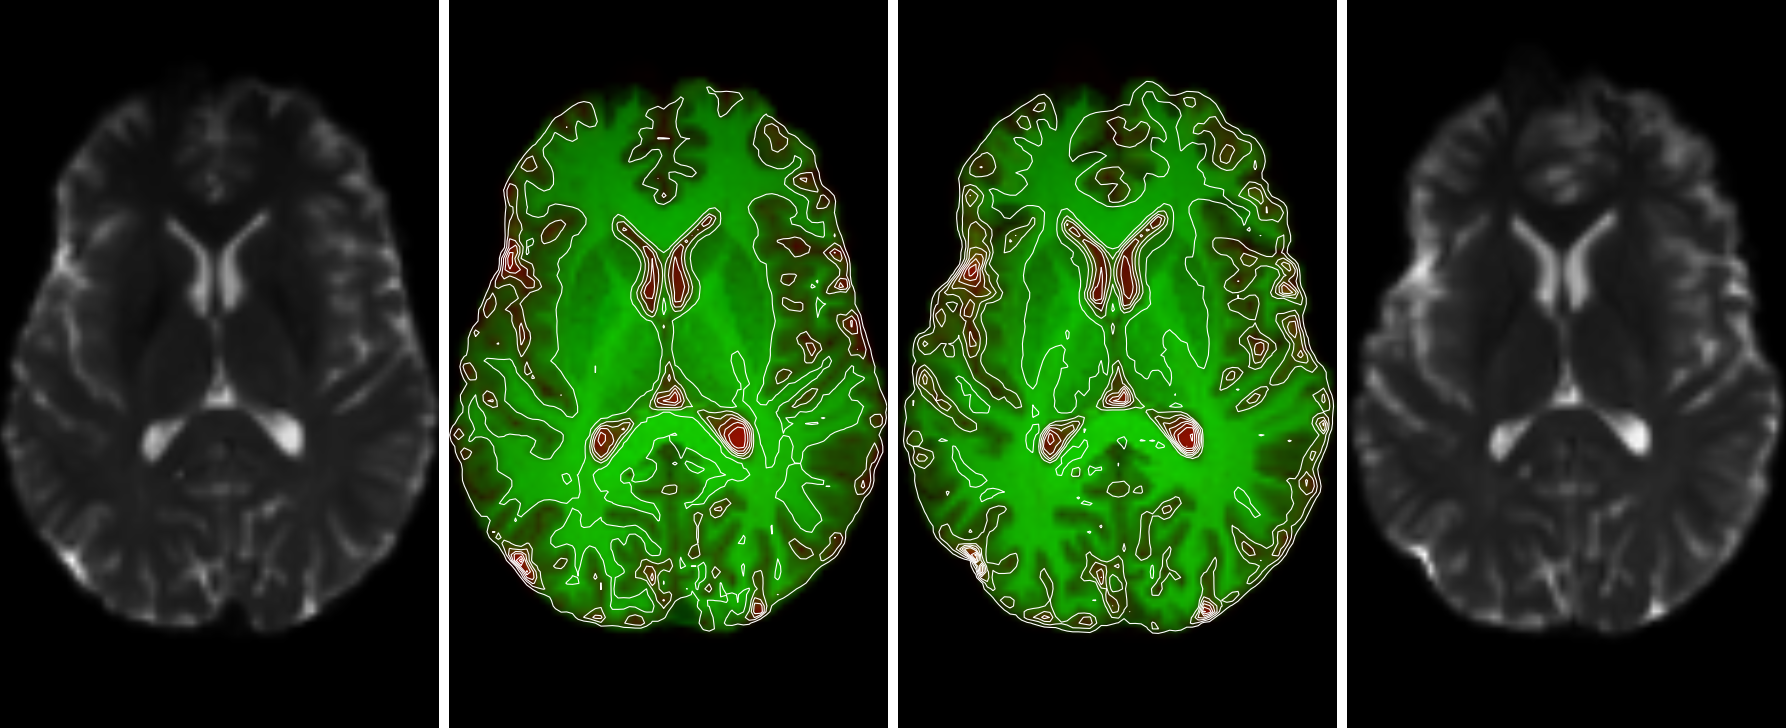
\includegraphics[width=1.0\linewidth]{./images/T1B0Result/epicor_b0up_ecc_mi.png}\\
    \caption{{\small Example of a $B_{0}$-T1 registration result using SyN with ECC (left) and MI (right). Level curves of the warped $B_{0}$ were overlaid on top of the (undeformed) T1 to visually assess local structure agreement. Visually, level curves obtained with ECC have a better correspondence with the structure of the T1. This visual assessment is confirmed quantitatively, as shown in fig. \ref{fig:indirect_validation_boxplots}.}}
\label{fig:comparison_B0_T1_coregistration}
\end{figure}

Since a realistic T1-$B_{0}$ template is not available, the validation methodology described in previous section cannot be used to validate $B_{0}$-T1 registration. Instead, we performed an indirect quantitative validation illustrated in Fig. \ref{fig:indirect_validation}. Here, we used the fact that the computed transformations are diffeomorphic. We first register the $B_{0}$ (moving) image towards each T1 (fixed) annotated image. Then, for every pair of T1-$B0$ transforms, we compute the composition (which now maps two annotated T1 images), warp one image towards the other and compute the Jaccard index of overlapping anatomical regions. The resulting overlap index indirectly measures the accuracy of both $B_{0}$-T1 registrations (although accumulating their errors) because a perfect multi-modal registration algorithm, should perfectly match both T1 images, even indirectly through the $B_{0}$, while the registration errors of one transform are unlikely to get ``fixed'' by the other after composition.
\begin{figure}[H]
\centering
    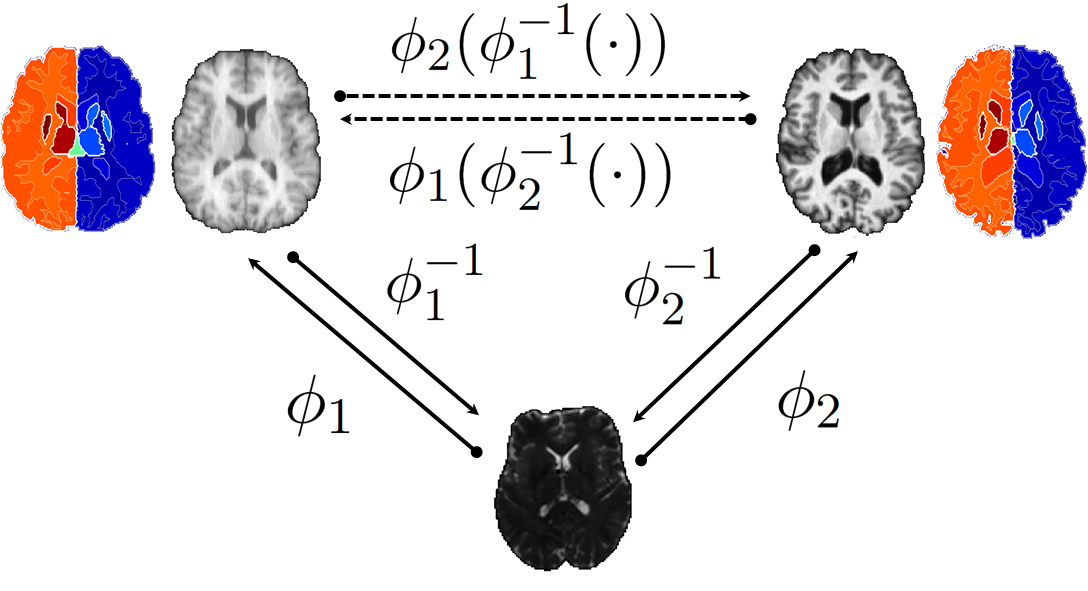
\includegraphics[width=\linewidth]{./images/new_validation.png}
    \caption{{\small Indirect validation protocol for $B_{0}$-T1 registration.}}
\label{fig:indirect_validation}
\end{figure}

Quantitative results of the indirect validation are depicted in fig. \ref{fig:indirect_validation_boxplots}. We can see that the average Jaccard index obtained with ECC is higher (and with lower variance) than using any of the other matching functionals, which also demonstrates the ECC robustness.
\begin{figure}[H]
\centering
    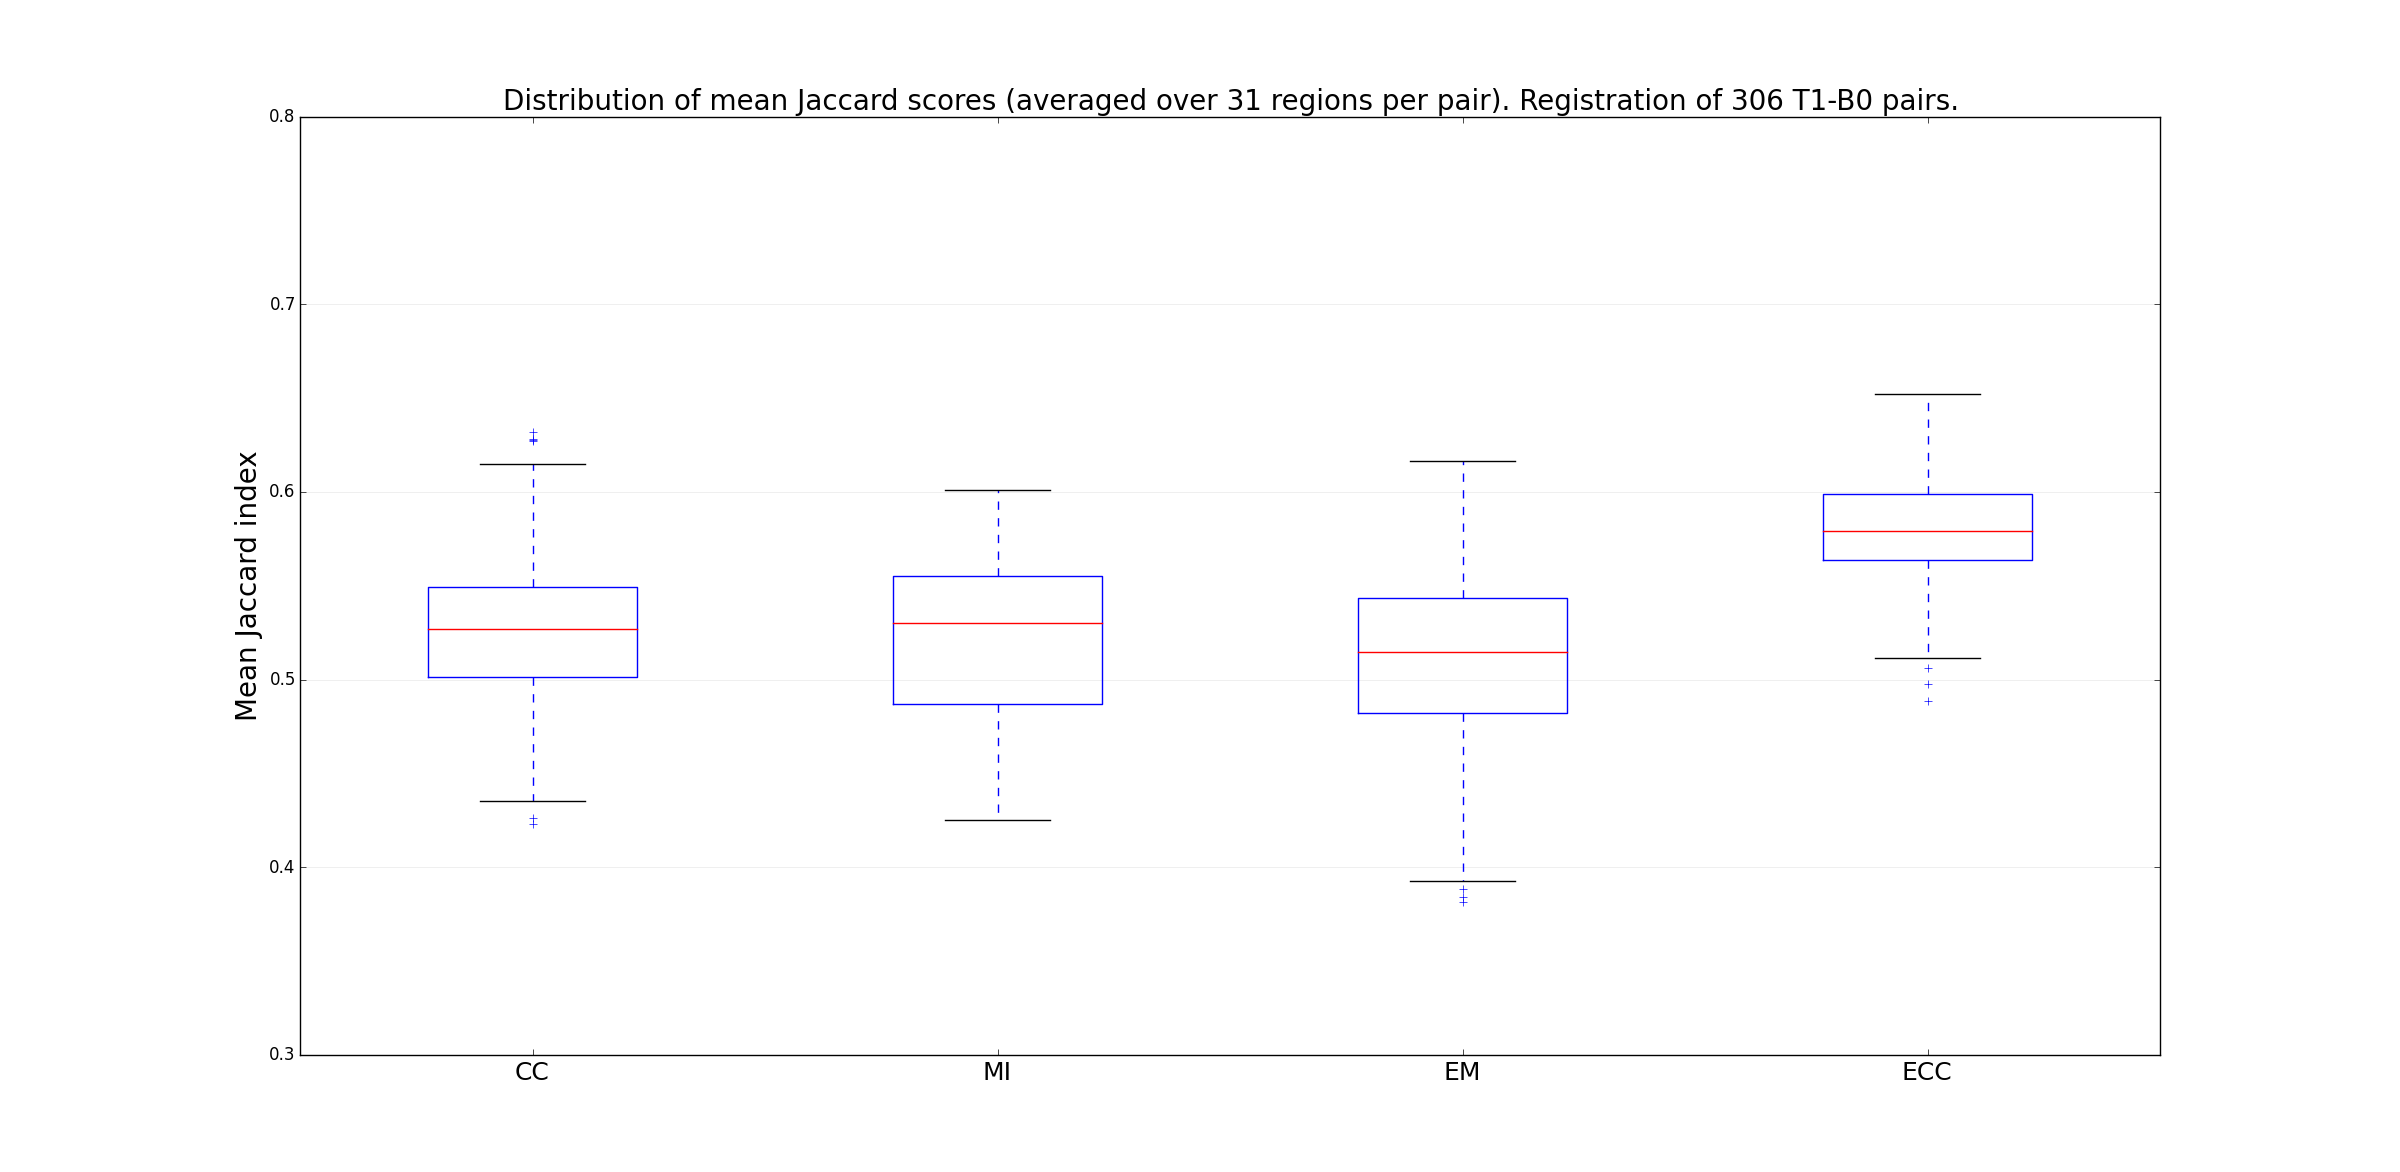
\includegraphics[width=\linewidth]{./images/T1B0Result/jaccard_boxplots_T1_B0.png}
    \caption{{\small $B0$-T1 registration results according to the validation procedure depicted in fig. \ref{fig:indirect_validation}.}}
\label{fig:indirect_validation_boxplots}
\end{figure}

\section{Discussion}
The matching functional presented in this work reduces the multi-modal problem to the mono-modal case by estimating two transfer functions between the two modalities. The main novelties introduced by our functional are: 1) it models the registration problem symmetrically, which allows us to use both transfer functions instead of selecting one of them arbitrarily, and 2) it computes two global transfer functions that makes the local relationship between image modalities as close to affine as possible. The estimation of both transfer functions is naturally introduced into the formulation of the SyN transformation model developed by Avants {\it et al.}\cite{Avants2008, Avants2011}, which may be regarded as a Generalized EM algorithm (GEM) \citep{Neal1998}, in which the energy is not fully optimized at each step with respect to the transformations $\phi_{I}, \phi_{J}$, but only reduced at each iteration. It has been shown that a full optimization in the maximization step is not necessary, and a local maximum of the likelihood is still reached with partial optimizations \citep{Neal1998}. The greedy SyN algorithm performs two displacement field inversions at each iteration (lines 7, 8 of algorithm \ref{alg:Greedy_SyN}), which may be regarded as projections to the space of diffeomorphisms. It is important to note that by directly inverting the displacement fields (using a variation of Chen's algorithm \cite{Chen2008}), the resulting transformations will be diffeomorphisms \footnote{Approximately diffeomorphisms, since there will always be numerical precision issues, regardless of how the inverse consistency is promoted.}\cite{Avants2008, Avants2011}. Therefore, it is unnecessary to introduce any constraint on the local Jacobians to ensure inverse consistency. Technically, it would be necessary to show that the two inversions effectively produce the projection of the updated displacement field to the space of diffeomorphisms, that way the optimization process of SyN might be interpreted as a gradient projection method \citep{Xiu2007}. However, the transformation model is not a contribution of this work, but only the matching functional for multi-modal registration.\\

The validation protocol using semi-synthetic images, proposed in this work allows us to quantitatively assess the accuracy of multi-modal registration algorithms under realistic conditions for three different image modalities and their combinations: T1, T2 and PD. It is very important to note that, although the way we generate the semi-synthetic images may appear to be tailored towards our model (applying a transfer function to the real T1 images), in other words, the so-called ``inverse crime'' that may bias the results towards the proposed method, this is not the case. Please note that in order to generate a semi-synthetic image, we compute a transfer function mapping intensities from each real T1 image to intensities of the warped T2/PD template (i.e. intensities of each real image are transformed using a different transfer function, independent from each other). Afterwards, the warped template is simply discarded, and not used for evaluation any more (it was used just to obtain a ``realistic'' transfer function). Images from the same subject (real and synthetic) are never registered to each other during evaluation. Therefore, there does not exist, in general, any transfer function mapping intensities between any pair of images registered during validation, which means that our model does not have any advantage under the proposed evaluation. Still, we did not exploit the full potential of this validation protocol: it is also possible to study the performance of the same multi-modal registration algorithms in the presence of noise and spatial inhomogeneities, since the Brainweb template allows us to realistically simulate this kind of distortions. A more comprehensive comparison of other available non-linear multi-modal algorithms including these artifacts is a subject for future research. For the full validation, it was necessary to perform 2,754 registrations for each of the 4 methods under evaluation (a total of 11,016 registrations). Finally, The lack of annotated data sets containing T1 and Diffusion images from the same subjects didn't allow us to quantitatively validate our matching functional for $B_{0}$-T1 co-registration. Still, the indirect quantitative validation we performed (containing only real data) allows us to assess the registration of $B_{0}$ and $T1$ images (although not from the same subject).\\

%It is important to note that, even though the proposed matching functional compared favourably against the other functionals under test for $B_{0}$-T1 registration, that doesn't mean that it is accurate enough to be used for correction of susceptibility induced geometric distortions, since quantitative evaluation only measures accuracy over relatively large anatomical regions.\\

\section{Conclusion}
We presented a new matching functional, which we call Expected Cross Correlation (ECC), for multi-modal image registration. We evaluated our matching functional using the publicly available IBSR database following the methodology of Klein {\it et al.}\cite{Klein2009, Klein2010} and Rohlfing \cite{Rohlfing2012} to show that it is competitive for mono-modal image registration. To evaluate the performance of ECC for multi-modal registration in a realistic, controlled, experiment we used the Brainweb \citep{Cocosco1997, Kwan1999} template to generate synthetic T2 and PD images for each of the IBSR T1 volumes. Experiments show that the CC metric is dramatically affected by the change of modality while the performance of ECC is less affected, remaining comparable to the mono-modal case and comparing favourably to the reference implementation of SyN with Mutual Information provided by the ANTS software. Our algorithms are publicly available in DIPY \citep{Garyfallidis2014}.\\


\section{Acknowledgements}
This work was supported in part by CONACYT, Mexico: research grants (324825, 131369 and 169178-F).


\appendix{Appendices}
\section{Computation of the E-Step}\label{ap:E_step}
Here, we show the details to compute the E-step of the EM algorithm \citep{Dempster1977} to obtain a local maximum likelihood estimator for $\Phi = (\phi_{I}, \phi_{J})$.
We follow similar steps as \cite{Arce-santana2014}.\\

The E-step \citep{Dempster1977} consists in computing the conditional expectation of the log-likelihood of the (complete) data $(Y, Z, \tilde{I}, \tilde{J}, \Phi)$, according to the observation model given in eq. \eqref{eq:SyNEM_gom_update}, where $Y, Z$ are hidden random fields modeling the (unknown) transfer functions between both modalities \hbox{(eq. \eqref{eq:hidden_fields})}. A consequence of the transformations $\phi_{I}, \phi_{J}$ being diffeomorphisms (in particular, invertible) is that the domains $\Omega_{I}, \Omega_{J}$ satisfy \hbox{$\phi_{I}(\Omega_{I}) = \Omega_{R} = \phi_{J}(\Omega_{J})$} (see Fig. \ref{fig:syn_overview}). This implies that $\tilde{I}$ is independent from $\phi_{I}$, because the event $\left\lbrace I(\phi_{I}^{-1}(x)) : x\in \Omega_{R} \right\rbrace$ is equal to the event $\left\lbrace I(y) : y\in \Omega_{I} \right\rbrace$, therefore:
\begin{equation}\label{eq:image_transform_independence}
     P(\tilde{I} | \Phi) = P(I | \Phi) = P(I).
\end{equation}
It is possible to obtain a similar independence property by making a weaker (injectivity, not necessarily invertibility) assumption \citep[see][pg. 73]{Roche2000}\\

We will assume that, when the transformations $\Phi=(\phi_{I}, \phi_{J})$ are known, the random fields $(Y, \tilde{I})$ are independent from $(Z, \tilde{J})$. In other words, once we know $\Phi$, any knowledge of $(Z, \tilde{J})$ no longer provide any additional information regarding the distribution of $(Y, \tilde{I})$, and viceversa. More precisely:
\begin{equation}\label{eq:conditional_independence_assumption}
    P(\tilde{I}, \tilde{J}, Y, Z | \Phi) = P(\tilde{I}, Y | \Phi)P(\tilde{J}, Z| \Phi).
\end{equation}
From eq. \eqref{eq:image_transform_independence}, it follows that
\begin{equation}\label{eq:joint_to_conditional}
    P(\tilde{I}, Y | \Phi) = P(Y | \tilde{I}, \Phi)P(\tilde{I} | \Phi) = P(Y | I, \Phi)P(I),
\end{equation}
similarly, $P(\tilde{J}, Z| \Phi) = P(Z| J, \Phi)P(J)$. From eqs. \eqref{eq:conditional_independence_assumption} and \eqref{eq:joint_to_conditional} we obtain
\begin{equation}\label{eq:simplified_joint_prob}
    P(\tilde{I}, \tilde{J}, Y, Z, \Phi) = P(Y | I, \Phi)P(Z| J, \Phi)P(\Phi)P(I)P(J).
\end{equation}

The conditional expectation of the log-likelihood (of the complete data) evaluated on an initial parameter $\Phi^{(0)}$ can be simplified using eq. \eqref{eq:simplified_joint_prob} as follows:
\begin{displaymath}
    Q(\Phi; \Phi^{(0)}) := \mathbbm{E}\left[\left. \log \left(P(\tilde{I}, \tilde{J}, Y, Z, \Phi)\right) \right | I, J, \Phi^{(0)}\right] =
\end{displaymath}
\begin{displaymath}
    \mathbbm{E}\left[\left. \log \left(P(Y |I, \Phi)P(Z|J, \Phi)P(\Phi)P(I)P{J}\right) \right | I, J, \Phi^{(0)}\right] =
\end{displaymath}
\begin{equation}\label{eq:separated_expectations}
    -R(\Phi) + C + \mathbbm{E}\left[ \log \left(P(Y|I, \Phi)\right) | I, J, \Phi^{(0)}\right] + \mathbbm{E}\left[ \log \left(P(Z|J, \Phi)\right) | I, J, \Phi^{(0)}\right]
\end{equation}
where $R(\Phi) = -\log P(\Phi)$ is known as the ``regularization term'', and \hbox{$C=\log \left(P(I)P(J)\right)$} is a constant that does not depend on $\Phi$. For simplicity, we will elaborate on the first expectation only, the second can be computed analogously.\\

By definition, the random field $\eta_{J}$ is a set of independent, zero-mean, Normally-distributed random variables. More precisely, if $f_{x}:\mathbf{R}\rightarrow \mathbf{R}^{+}$ is the probability density
function of $\eta_{J}(x)$ then:
\begin{equation}\label{eq:gaussian}
    f_{x}(u) = \frac{1}{\sigma_{Y}(x)\sqrt{2 \pi}}\exp\left(-\frac{u^{2}}{2\sigma^{2}_{Y}(x)}\right)
\end{equation}
and, from our observation model (eq. \eqref{eq:SyNEM_gom_update}), it follows that:
\begin{equation}
    P(Y(x)| I, \Phi) = P(\eta_{J}(x) = Y(x)-\tilde{I}(x)) = f_{x}(Y(x)-\tilde{I}(x)).
\end{equation}
Therefore, the joint conditional probability of $Y$ given $I, \Phi$ is the product of the above marginals:
\begin{equation}\label{eq:Y_field_cond_indep}
    P(Y|I, \Phi) = \prod_{x\in{\Omega_{R}}} f_{x}(Y(x) - \tilde{I}(x)),
\end{equation}
and the first conditional expectation of eq. \eqref{eq:separated_expectations} can be writen as:
\begin{equation}
    Q_{I}(\phi_{I} ; \Phi^{(0)}) := \int_{\mathcal{Y}}\left[\sum_{x\in\Omega_{R}} \log f_{x}\left(y(x) - \tilde{I}(x)\right) \right] dP(y | I, J, \Phi^{(0)}),
\end{equation}
where $\mathcal{Y}$ is the set of all possible configurations of the vector field $Y$. By assuming a finite grid $\Omega_{R}$, we may interchange the order of summation and integration, which yields:
\begin{equation}\label{eq:data_term}
    Q_{I}(\phi_{I} ; \Phi^{(0)}) = \sum_{x\in\Omega_{R}} \int_{\mathcal{Y}} \log f_{x}\left(y(x) - \tilde{I}(x)\right)  dP(y | I, J, \Phi^{(0)}).
\end{equation}

Since all the variables $Y(x), x\in\Omega_{R}$ are conditionally independent given $I, \Phi^{(0)}$ (eq. \eqref{eq:Y_field_cond_indep}), we have $P(y | I, J, \Phi^{(0)}) = P(y(x)| I, J, \Phi^{(0)})P(y^{C}(x) | I, J, \Phi^{(0)})$, where the complement $Y^{C}(x)$
denotes the subset of random variables other than $Y(x)$, and $y^{C}(x)$ is a configuration of $Y^{C}(x)$. Therefore, the right-hand side of eq.\eqref{eq:data_term} can be written as

\begin{equation}\label{eq:split_integral}
    \sum_{x\in\Omega_{R}} \int_{\mathcal{Y}^{C}(x)} \left[\int_{\mathbf{R}} \log f_{x}\left(\ell - \tilde{I}(x)\right) P(Y(x) = \ell | I, J, \Phi^{(0)})d\ell\right]  dP(y^{C}(x) | I, J, \Phi^{(0)})
\end{equation}
where $\mathcal{Y}^{C}(x)$ is the set of all possible configurations of $Y^{C}(x)$.\\

Since \hbox{$\int_{\mathcal{Y}^{C}(x)}dP(y^{C}(x) | I, J, \Phi^{(0)}) = 1$}, and the inner integral
is an expected value w.r.t. the conditional distribution:
\begin{equation}
     Q_{I}(\phi_{I} ; \Phi^{(0)}) = \sum_{x\in\Omega_{R}} \mathbbm{E} \left[\left.\log f_{x}\left(Y(x) - \tilde{I}(x)\right) \right| I, J, \Phi^{(0)}\right].
\end{equation}
By expanding the density function (according to eq. \eqref{eq:gaussian}) and denoting by $\overline{Y}(x), \widehat{\sigma^{2}_{Y}(x)}$ the conditional mean and variance of $Y(x)$
given the data and fixed parameters $\Phi^{(0)}$, we have
\begin{equation}
    \mathbbm{E} \left[\left.\log \frac{1}{\sigma_{Y}(x)\sqrt{2\pi}} - \frac{(Y(x) - I(\phi^{-1}_{I}(x)))^{2}}{2\sigma^{2}_{Y}(x)}\right|I, J, \Phi^{(0)} \right] =
\end{equation}
\begin{equation}
    = \log \frac{1}{\sigma_{Y}(x)\sqrt{2\pi}} - \mathbbm{E} \left[\left. \frac{(Y(x) - \overline{Y}(x) + \overline{Y}(x) - I(\phi^{-1}_{I}(x)))^{2}}{2\sigma^{2}_{Y}(x)}\right|I, J, \Phi^{(0)} \right]=
\end{equation}
%\begin{equation}
%    = \log \frac{1}{\sigma_{Y}(x)\sqrt{2\pi}} - \mathbbm{E} \left[\left. \frac{(Y(x) - \overline{Y}(x))^{2}+ (\overline{Y}(x) - I(\phi^{-1}_{I}(x)))^{2} - 2(Y(x) - \overline{Y}(x)) (\overline{Y}(x) - I(\phi^{-1}_{I}(x)))}{2\sigma^{2}_{Y}(x)}\right|I, J, \Phi^{(0)} \right]=
%\end{equation}
\begin{equation}
    = \log \frac{1}{\sigma_{Y}(x)\sqrt{2\pi}} - \frac{\widehat{\sigma^{2}_{Y}(x)} + (\overline{Y}(x) - I(\phi^{-1}_{I}(x)))^{2}}{2\sigma^{2}_{Y}(x)}.
\end{equation}
Finally, by approximating the (unknown) parameters $\sigma_{Y}(x)$ by $\widehat{\sigma_{Y}(x)}$ we obtain:
\begin{equation}
    Q_{I}(\phi_{I} ; \Phi^{(0)}) = C_{I} - \sum_{x\in\Omega_{x}}\frac{(\overline{Y}(x) - I(\phi^{-1}_{I}(x)))^{2}}{2\widehat{\sigma^{2}_{Y}(x)}},
\end{equation}
where $C_{I} = -\frac{1}{2} - \log\left(\widehat{\sigma^{2}_{Y}(x)}\sqrt{2\pi}\right)$ is a constant that depends on the (known) initial transformations $\Phi^{(0)}$, but not on the (unknown) transformation $\phi_{I}$ we wish to optimize. Image $\overline{Y}$ may be regarded as an approximation of image $\tilde{I}$, since it can be efficiently computed by assigning to $\overline{Y}(x)$ the average intensity of the iso-set $\left\lbrace \tilde{I}(y) : \tilde{J}(y) = \tilde{J}(x)\right\rbrace$ \citep{Roche1998}. The conditional variance $\widehat{\sigma^{2}_{Y}}(x)$ measures the uncertainty at each point $x\in \Omega_{R}$.\\

Similarly, if $\overline{Z}(x), \widehat{\sigma^{2}_{Z}(x)}$ are the conditional mean and variance of $Z(x)$ given the data
and fixed parameters $\Phi^{(0)}$, the second conditional expectation of eq. \eqref{eq:separated_expectations} can be writen as

\begin{equation}
    Q_{J}(\phi_{J}; \Phi^{(0)}) = C_{J} - \sum_{x\in\Omega_{x}}\frac{(\overline{Z}(x) - J(\phi^{-1}_{J}(x)))^{2}}{2\widehat{\sigma^{2}_{Z}(x)}}.
\end{equation}
If we choose a regularization function of the form $R(\Phi) = \lambda R_{I}(\phi_{I}) + \lambda R_{J}(\phi_{J})$ the final function to be \textbf{maximized} in the M step is given by

\begin{equation}
    Q(\Phi; \Phi^{(0)}) = \left[Q_{I}(\phi_{I}; \Phi^{(0)}) - \lambda R_{I}(\phi_{I})\right] + \left[Q_{J}(\phi_{J}; \Phi^{(0)}) - \lambda R_{J}(\phi_{J})\right],
\end{equation}
which is the sum of two independent cost functions for $\phi_{I}$ and $\phi_{J}$.

\section{Gradient of the CC metric}\label{ap:CC_gradient}
We are interested in computing the gradient of
\begin{equation}
    CC(\bar{I}, \bar{J}, x) = \frac{<\bar{I}, \bar{J}>^{2}}{<\bar{I}><\bar{J}>}
\end{equation}
where the inner product is taken over an $n^{D}$ window \citep[see][eq. 4]{Avants2008}. Since the windows are considered discrete, a more precise notation
for this expression is:
\begin{equation}\label{eq:CC_definition}
    CC(y;\phi_{I}, \phi_{J}) = \frac{\left[\sum_{z\in W_{y}} \left(\tilde{I}(z) - \mu_{y}\right)\left(\tilde{J}(z) - \nu_{y}\right)\right]^{2}}
    {\left[\sum_{z \in W_{y}}\left(\tilde{I}(z) - \mu_{y}\right)^{2}\right] \left[\sum_{z \in W_{y}}\left(\tilde{J}(z) - \nu_{y}\right)^{2}\right]} = \frac{A_{y}^{2}}{B_{y}C_{y}}
\end{equation}
where $\tilde{I}(z) = I(\phi_{I}^{-1}(z))$, $\tilde{J}(z) = J(\phi_{J}^{-1}(z))$ and the full energy is given by
\begin{equation}
    CC(\phi_{I}, \phi_{J}) = \sum_{y\in\Omega} CC(y; \phi_{I}, \phi_{J})
\end{equation}
where $W_{y}$ is the window of side $n$ centered at voxel $y$, $|W_{y}|$ is the number of voxels in window $W_{y}$ and:
\begin{equation}
    \begin{array}{lll}
        \mu_{y} &=& \frac{1}{|W_{y}|}\sum_{z \in W_{y}}\tilde{I}(z)\\[+2mm]
        \nu_{y} &=& \frac{1}{|W_{y}|}\sum_{z \in W_{y}}\tilde{J}(z)\\
    \end{array}.
\end{equation}

We wish to compute the gradient of $CC(\phi_{I}, \phi_{J})$ with respect to $\phi^{-1}_{J}(x)$, $x\in\Omega$. The set of window terms $CC(y;\phi_{I}, \phi_{J})$
that depend on $\phi^{-1}_{J}(x)$ is precisely the set of all windows $W_{y}$ such that $y \in W_{x}$. Therefore:
\begin{equation}
    \frac{\partial CC (\phi_{I}, \phi_{J})}{\partial \phi^{-1}_{J}(x)} = \sum_{y \in W_{x}} \frac{\partial CC (y; \phi_{I}, \phi_{J})}{\partial \phi^{-1}_{J}(x)}
\end{equation}
and
\begin{equation}
    \frac{\partial CC (y; \phi_{I}, \phi_{J})}{\partial \phi^{-1}_{J}(x)} =
        \frac{\left(2A_{y} B_{y}C_{y}\right)\frac{\partial A_{y}}{\partial \phi^{-1}_{J}(x)} - \left(A_{y}^{2}B_{y}\right)\frac{\partial C_{y}}{\partial \phi^{-1}_{J}(x)}}
             {B_{y}^{2} C_{y}^{2}}
\end{equation}
where
\begin{equation}
    \begin{array}{lll}
        \frac{\partial A_{y}}{\partial \phi^{-1}_{J}(x)} &=& (\tilde{I}(x) - \mu_{y})\nabla \tilde{J}(x)\\[+3mm]
        \frac{\partial C_{y}}{\partial \phi^{-1}_{J}(x)} &=& 2(\tilde{J}(x) - \nu_{y})\nabla \tilde{J}(x)
    \end{array}.
\end{equation}
After simplifying, we get
\begin{equation}\label{eq:CC_gradient}
    \frac{\partial CC (\phi_{I}, \phi_{J})}{\partial \phi^{-1}_{J}(x)} = \sum_{y \in W_{x}}
         \frac{2A_{y}}
              {B_{y}C_{y}}\left[ (\tilde{I}(x) - \mu_{y}) - \frac{A_{y}}{C_{y}}\left(\tilde{J}(x) - \nu_{y}\right)\right]\nabla \tilde{J}(x).
\end{equation}
If we define the scalar functions
\begin{equation}
    \begin{array}{lll}
        S_{a}(x) &=& \sum_{y \in W_{x}} \frac{2A_{y}}{B_{y}C_{y}}\\[+2mm]
        S_{b}(x) &=& \sum_{y \in W_{x}} \frac{2A_{y}^{2}}{B_{y}C_{y}^{2}}\\[+2mm]
        S_{c}(x) &=& \sum_{y \in W_{x}} \frac{2A_{y}}{B_{y}C_{y}} \left[ \mu_{y} - \frac{A_{y}}{C_{y}}\nu_{y}\right].
    \end{array}
\end{equation}
we can write the gradient of $CC$ with respect to $\phi^{-1}_{J}$ as:

\begin{equation}
    \psi_{J} = \nabla_{\phi^{-1}_{J}} CC(\phi_{I}, \phi_{J}) = \left[S_{a} \tilde{I} - S_{b}\tilde{J} - S_{c}\right]\nabla \tilde{J}.
\end{equation}

It is important to notice the similarity and differences between equation \eqref{eq:CC_gradient} and the expressions derived by \cite{Hermosillo2004}
and \cite{Avants2008}. On the one hand, \cite{Hermosillo2004} considered separately the cases of local and global intensity comparisons: the global comparison corresponds to setting $W_{x} = \Omega$ (summing over the full domain). The local intensity comparison is accomplished by using a Gaussian kernel centered at each location $x\in\Omega$. The limitation of using Gaussian kernels is the computational cost, as pointed out by \cite{Hermosillo2004}, which makes it necessary to perform some simplifications and use parallel computing, while using rectangular windows results in a very efficient and robust implementation, as shown by \cite{Avants2008}. On the other hand, even though the formulation of \cite{Avants2008} is the same as eq. \eqref{eq:CC_definition}, only the central voxel contributes to the sum in eq. \eqref{eq:CC_gradient} \citep[see][eqs. 6, 7]{Avants2008}. In practice, we have not observed significant differences between the quantitative results using eq. \eqref{eq:CC_gradient} of this appendix, and eqs. (6) and (7) from \cite{Avants2008}, thus we opted for using rectangular windows and the gradient computations as in \cite{Avants2008}.

\section{Algorithms}\label{ap:Algorithms}
\begin{algorithm}[h!]
\caption{Greedy SyN. This algorihtm was the method used for evaluating ANTS \citep{Avants2011} in the large comparative studies developed by \cite{Klein2009, Klein2010} in which it consistently ranked first.}\label{alg:Greedy_SyN}
\begin{algorithmic}[1]
\REQUIRE Gaussian kernel parameter $\sigma>0$
\REQUIRE Step size $\epsilon>0$
\REQUIRE Maximum number of iterations $T>0$
\STATE Initialize: $\phi_{i}(\cdot, 0.5) = Id, i=1, 2$
\STATE $t=0$
\REPEAT
    \STATE Warp $\tilde{I}  = I \circ \phi_{1}^{-1}(\cdot, 0.5), \tilde{J} = J \circ \phi_{2}^{-1}(\cdot, 0.5)$
    \STATE Compute the gradients $\mathbf{u}_{i} = \nabla_{\phi_{i}} \Pi(\tilde{I}, \tilde{J}), i=1,2$
%    \STATE Update $\phi_{i}(\cdot, 0.5), i=1, 2$ according to eq. \eqref{eq:gsyn_update}
    \STATE Update $\phi_{i}(\cdot, 0.5) = \phi_{i}(\cdot, 0.5) - \left( \epsilon K_{\sigma} \ast \mathbf{u}_{i} \right) \circ \phi_{i}(\cdot, 0.5)$
    \STATE Invert $\phi_{i}^{-1}(\cdot, 0.5) = invert (\phi_{i}(\cdot, 0.5)), i=1, 2$
    \STATE Invert $\phi_{i}(\cdot, 0.5) = invert (\phi_{i}^{-1}(\cdot, 0.5)), i=1, 2$
    \STATE t = t + 1
\UNTIL{$t\geq T$ or convergence}
\RETURN $\phi_{i}(\cdot, 0.5), i=1,2$
\end{algorithmic}
\end{algorithm}


\begin{algorithm}[h!]
\caption{SyN-EM. This algorithm uses a symmetric extension of the EM metric proposed by \cite{Arce-santana2014}.}\label{alg:SyNEM}
\begin{algorithmic}[1]
\REQUIRE Gaussian kernel parameter $\sigma>0$
\REQUIRE Step size $\epsilon>0$
\REQUIRE Maximum number of iterations $T>0$
\STATE Initialize: $\phi_{I} = Id, \phi_{J} = Id$
\STATE $t=0$
\REPEAT
    \STATE Warp $\tilde{I}  = I \circ \phi_{I}^{-1}, \tilde{J} = J \circ \phi_{J}^{-1}$
    \STATE E-Step (eq. \eqref{eq:expectation_transfer}) $\overline{Y}(x) = \mathbbm{E}\left[\left.\mathbf{I}\right| \mathbf{J}= J(\phi_{J}^{-1}(x))\right]$
    \STATE E-Step $\overline{Z}(x) = \mathbbm{E}\left[\left.\mathbf{J}\right| \mathbf{I}= I(\phi_{I}^{-1}(x))\right]$
    \STATE E-Step (eq. \eqref{eq:expectation_variance}) $\sigma^{2}_{Y}(x) = Var\left[\left.\mathbf{I}\right| \mathbf{J}= J(\phi_{J}^{-1}(x))\right]$
    \STATE E-Step $\sigma^{2}_{Z}(x) = Var\left[\left.\mathbf{J}\right| \mathbf{I}= I(\phi_{I}^{-1}(x))\right]$
    \STATE M-Step (eq. \eqref{eq:euler_lagrange_step1}) $\mathbf{u}_{I} = \frac{\overline{Y}(x) - \tilde{I}(x)}{||\nabla \tilde{I}(x)||^{2} + \frac{\sigma_{Y}^{2}(x)}{\tau}}\nabla \tilde{I}(x)$
    \STATE M-Step $\mathbf{u}_{J} = \frac{\overline{Z}(x) - \tilde{J}(x)}{||\nabla \tilde{J}(x)||^{2} + \frac{\sigma_{Z}^{2}(x)}{\tau}}\nabla \tilde{J}(x)$
    \STATE Update $\phi_{I} = \phi_{I} - \left(\epsilon K_{\sigma} \ast \mathbf{u}_{I} \right)\circ \phi_{I}$
    \STATE Update $\phi_{J} = \phi_{J} - \left(\epsilon K_{\sigma} \ast \mathbf{u}_{J} \right)\circ \phi_{J}$
    \STATE Invert $\phi_{I}^{-1}, \phi_{J}^{-1} = invert(\phi_{I}), invert(\phi_{J})$
    \STATE Invert $\phi_{I}, \phi_{J} = invert(\phi_{I}^{-1}), invert(\phi_{J}^{-1})$
    \STATE t = t + 1
\UNTIL{$t\geq T$ or convergence}
\RETURN $\phi_{I}, \phi_{J}$
\end{algorithmic}
\end{algorithm}


\begin{algorithm}[h!]
\caption{SyN-ECC. This algorithm uses an extension of the CC metric for multi-modal images. It uses a (global) estimation of the transfer functions between the two image modalities and measures the similarity of (local) image windows with the CC metric.}\label{alg:SyNECC}
\begin{algorithmic}[1]
\REQUIRE Gaussian kernel parameter $\sigma>0$
\REQUIRE Step size $\epsilon>0$
\REQUIRE Maximum number of iterations $T>0$
\STATE Initialize: $\phi_{I} = Id, \phi_{J} = Id$
\STATE $t=0$
\REPEAT
    \STATE Warp $\tilde{I}  = I \circ \phi_{I}^{-1}, \tilde{J} = J \circ \phi_{J}^{-1}$
    \STATE E-Step (eq. \eqref{eq:expectation_transfer}) $\overline{Y}(x) = \mathbbm{E}\left[\left.\mathbf{I}\right| \mathbf{J}= J(\phi_{J}^{-1}(x))\right]$
    \STATE E-Step $\overline{Z}(x) = \mathbbm{E}\left[\left.\mathbf{J}\right| \mathbf{I}= I(\phi_{I}^{-1}(x))\right]$
    \STATE E-Step (eq. \eqref{eq:expectation_variance}) $\sigma^{2}_{Y}(x) = Var\left[\left.\mathbf{I}\right| \mathbf{J}= J(\phi_{J}^{-1}(x))\right]$
    \STATE E-Step $\sigma^{2}_{Z}(x) = Var\left[\left.\mathbf{J}\right| \mathbf{I}= I(\phi_{I}^{-1}(x))\right]$
    \STATE M-Step (gradient of eq. \eqref{eq:ecc_metric}) $\mathbf{u}_{I} = - \nabla_{\phi^{-1}_{I}} ECC(\tilde{I}, \tilde{J} | \phi_{I}, \phi_{J})$
    \STATE M-Step $\mathbf{u}_{J} = - \nabla_{\phi^{-1}_{J}} ECC(\tilde{I}, \tilde{J} | \phi_{I}, \phi_{J})$
    \STATE Update $\phi_{I} = \phi_{I} - \left(\epsilon K_{\sigma} \ast \mathbf{u}_{I} \right)\circ \phi_{I}$
    \STATE Update $\phi_{J} = \phi_{J} - \left(\epsilon K_{\sigma} \ast \mathbf{u}_{J} \right)\circ \phi_{J}$
    \STATE Invert $\phi_{I}^{-1}, \phi_{J}^{-1} = invert(\phi_{I}), invert(\phi_{J})$
    \STATE Invert $\phi_{I}, \phi_{J} = invert(\phi_{I}^{-1}), invert(\phi_{J}^{-1})$
    \STATE t = t + 1
\UNTIL{$t\geq T$ or convergence}
\RETURN $\phi_{I}, \phi_{J}$
\end{algorithmic}
\end{algorithm}

\clearpage
\section*{References}
\bibliographystyle{model2-names}
\bibliography{references}

\clearpage
\section*{Vitae}
\textbf{Omar Ocegueda} received the B.S. degree in Computer Science in 2004 from the University of Guanajuato, Mexico and the M.S. degree in Computer Science and Industrial Mathematics from the Center for Research in Mathematics (CIMAT), Guanajuato, Mexico in 2006. He is currently a PhD student at CIMAT working on computational methods for diffusion MRI processing. His main research interests include image processing, optimization, and machine learning.\\

\textbf{Eleftherios Garyfallidis} received the B.Sc. degree in Computer Science from the Technological Institution of Athens, Athens, Greece, in 2003, and the M.Sc. degree in Brain and Mind Sciences from the University of Crete and the Foundation for Research and Technology Hellas (FORTH), Crete, Greece, in 2006. In 2012, he received  the Ph.D. degree from the University of Cambridge, Cambridge, United Kingdom. He is currently a Post-doctoral Fellow at the Shebrooke Connectivity Imaging Lab (SCIL), Computer Science department, the University of Sherbrooke, Sherbrooke, Canada.\\

\textbf{Pr. Maxime Descoteaux} is the head of the Sherbrooke Connectivity Imaging Lab (SCIL) and the scientific director of the image analysis and visualization plateform (PAVI) of the Centre de Recherche CHUS. He currently supervises 12 MSc, PhD and post-doctorat students. He did a post-doctorat at NeuroSpin, France under the supervision of Cyril Poupon. He also obtained a PhD in Computer Science at INRIA Sophia Antipolis - Mediterranée, France, supervised by R. Deriche. Finally, He obtained his M.Sc under the supervision of K. Siddiqi in Computer Science at Center for Intelligent Machines, McGill University, where he also obtained my B.Sc., graduating from the joint honors Mathematics and Computer Science program.\\

\textbf{Mariano Rivera} received the B.E. degree in electronics from the Durango Institute of Technology, Mexico, in 1989, the M.Sc. degree in electronics from the Chihuahua Institute of Technology, Mexico, in 1993, and the D.Sc. degree in optics from the Center for Research in Optics (CIO), Leon, Mexico, in 1997. Since 1997, he has been with the Computer Science Department, Center for Research in Mathematics (CIMAT), Guanajuato, Mexico. His current interests include computer vision, image processing, medical image analysis, machine learning, and optimization. His research is summarized in more than 80 papers in scientific journals and conference proceedings. Dr. Rivera is Fellow of the National Researcher System (SNI) of the Mexican Government.
\end{document}
